\defcitealias{ali_et_al2015}{A15}

\chapter{Power Spectrum Methods}
\label{c.PSmethods}

% change "Chapter" to "Chapter"

\section{Power Spectrum Themes and Techniques}

The major challenge that faces all 21\,cm experiments is isolating a small signal that is buried underneath foregrounds and 
instrumental systematics that are, when combined, four to five orders of magnitude brighter \citep[e.g.,][]{santos_et_al2005, ali_et_al2008, deOliveiraCosta_et_al2008, jelic_et_al2008, bernardi_et_al2009, bernardi_et_al2010, ghosh_et_al2011, pober_et_al2013b, bernardi_et_al2013, dillon_et_al2014, kohn_et_al2016}. A clean measurement therefore requires an intimate understanding of the instrument and a rigorous study of data analysis choices. With continual progress being made 
in the field and HERA on the horizon, it is becoming increasingly important to understand how the methods we choose interact 
with each other to affect power spectrum results. More specifically, it is imperative to develop techniques and tests that ensure 
the accuracy and reliability of a potential EoR detection. In this chapter and the next, we discuss three topics (signal loss, error estimation, and bias) that are essential to investigate 
for a robust 21\,cm power spectrum analysis. We also highlight four power spectrum techniques (fringe-rate filtering, weighting, bootstrapping, jackknife testing) and their trade-offs, potential 
pitfalls, and connections to the themes. We first approach the themes from a broad perspective (Chapter \ref{c.PSmethods}), introducing the themes of our focus and using toy models to develop intuition into each one. We then perform a detailed 
case study (Chapter \ref{c.PSA64}) using data from the 64-element configuration of PAPER, highlighting key changes from the methods used in the previously published result in \citet{ali_et_al2015}, henceforth known as \citetalias{ali_et_al2015}, which have led to a 
revised PAPER-64 power spectrum result. In these two chapters we use a subset of PAPER-64 data to illustrate our revised analysis methods, while Chapter \ref{c.PSA64_results} builds off of the methods to finally present revised PAPER-64 results for multiple redshifts and baseline types.

We note that this thesis as a whole adds to the growing foundations of lessons which have been documented, for example, in \citet{paciga_et_al2013}, \citet{Patil2016}, and \citet{jacobs_et_al2016}, by the GMRT, LOFAR, and MWA projects respectively. These lessons are imperative as the community as a whole moves towards higher sensitivities and potential EoR detections.

There are many choices a 21\,cm data analyst must consider. How can time-ordered measurements be combined? How can the 
variance of the data be estimated? In what way(s) can the data be weighted to suppress contaminated modes while not 
destroying an EoR signal? How can a statistically significant detection of a signal be properly identified? Many common techniques, such as 
averaging data, weighting, bootstrapping, and jackknife testing, address these issues but harbor additional trade-offs. For 
example, an aggressive filtering method may succeed in eliminating interfering systematics but comes at the cost of losing 
some EoR signal. A chosen weighting scheme may theoretically maximize sensitivity but fail to suppress foregrounds in practice. 

Though there are many data analysis choices, measuring the statistical 21\,cm power spectrum ultimately requires robust 
methods for determining accurate confidence intervals and rigorous techniques to identify and control systematics.  In this 
thesis, we focus on three 21\,cm power spectrum themes that encapsulate this goal and discuss four techniques that interplay 
with each other and impact the themes. We will give brief definitions now, and build intuition for each theme in the sections to 
follow.

\begin{itemize}
\item \textbf{Signal Loss} (Chapters \ref{sec:SiglossOverview} and \ref{sec:SiglossMath}): Signal loss refers to attenuation of the target \textit{cosmological} signal 
in a power spectrum estimate. Certain analysis techniques can cause this loss, and if the amount of loss is not quantified accurately, it could lead to false non-detections and overly aggressive upper limits. Determining whether an analysis pipeline is lossy, and estimating the amount of loss if so, has subtle challenges but is necessary to ensure the accuracy of any result. 
\item \textbf{Error Estimation} (Chapter \ref{sec:ErrorOverview}): Confidence intervals on a 21\,cm power spectrum result 
determine the difference between a detection and a null result, which have two very different implications. Additionally, accurate error estimation is crucial for the comparison of results to theoretical models. Errors can be 
estimated in a variety of ways, and we will discuss a few of them.
\item \textbf{Bias} (Chapter \ref{sec:BiasOverview}): There are several possible sources of power offset in a visibility 
measurement that can show up as a detection in a power spectrum, such as bias from noise and foregrounds. In particular, a 
successful EoR detection would also imitate a bias. Proving that a bias is an EoR detection may be the most difficult challenge for future 21\,cm 
analyses, as it is crucial to be able to distinguish a detection of foreground leakage, for example, from that of EoR. In this chapter,
we will highlight some sources of bias, discuss ways to mitigate their effects, and describe example tests that a true EoR detection must 
pass.
\end{itemize}

The following techniques each have advantages when it comes to maximizing sensitivity and understanding systematics in 
data. However, some have limitations, and we will discuss circumstances in which there are trade-offs. We choose to focus on 
these four techniques because they represent major steps in PAPER's power spectrum pipeline, with several of them also 
being standard steps in general 21\,cm analyses.
\begin{itemize}
\item \textbf{Fringe-rate filtering:} Fringe-rate filtering is an averaging scheme for time-ordered data 
(\citealt{parsons_et_al2016}). Broadly, a fringe-rate filter averages visibilities in time to produce a smaller number of more sensitive 
independent samples. However, such a filter also affects the presence 
of foregrounds and systematics. We explain the trade-offs of filtering in more detail in Chapter \ref{sec:toymodel_frf}.
\item \textbf{Weighting:} A dataset can be weighted to emphasize certain features and minimize others. One particular flavor of 
weighting employed by previous PAPER analyses is inverse covariance weighting in frequency, which is a generalized version of inverse variance 
weighting that also takes into account frequency correlations (\citealt{liu_tegmark2011}; \citealt{dillon_et_al2013a}; \citealt{liu_et_al2014a}; \citealt{liu_et_al2014b}; \citealt{dillon_et_al2014}; \citealt{dillon_et_al2015}). Using such a technique enables the down-weighting of contaminant modes that obey a different covariance structure from that of cosmological modes. However, a challenge of inverse covariance 
weighting is in estimating a covariance matrix that is closest to the true covariance of the data; the discrepancy between the two can have large impacts on signal loss. We investigate the impact of different types of weighting on signal loss in Chapter \ref{sec:SiglossOverview}.
\item \textbf{Bootstrapping:} In addition to using theoretical models for covariance matrices and theoretical error estimation 
methods, bootstrapping is one way to estimate errors. Namely, bootstrapping is a useful method for estimating errors of a dataset from 
itself (\citealt{andrae2010}). By randomly drawing many subsamples of the data, we obtain a sense of its inherent variance, though there are subtleties to 
consider such as the independence of values in a dataset. We explore this potential pitfall of bootstrapping in Chapter \ref{sec:ErrorOverview}.
\item \textbf{Jackknife testing:} A resampling technique useful for estimating bias, jackknives can be taken along different 
dimensions of a dataset to cross-validate results. In particular, null tests can be used to verify whether results are free of 
systematics, as done with CO power spectra (\citealt{keating_et_al2016}) and CMB measurements (see e.g. \citealt{ade_et_al2008}; \citealt{chiang_et_al2010}; \citealt{bischoff_et_al2011}; \citealt{das_et_al2011b}; \citealt{araujo_et_al2012}; \citealt{crites_et_al2015}; \citealt{ade_et_al2016}; \citealt{ade_et_al2017}; \citealt{sherwin_et_al2017}). An EoR detection must pass both jackknife and null tests, which we highlight in Chapter \ref{sec:JackknifeOverview}.
\end{itemize}

In this chapter, we study each theme in depth, focusing on how power spectrum technique trade-offs affect each. 
We use toy data models to develop intuition into why certain analysis choices may be appealing and discuss ways in which 
they are limited. We highlight problems that can arise regarding each theme and offer suggestions to mitigate the issues. 
Ultimately, we show that rigorous investigations into signal loss, error estimation, and bias must be performed for robust 21\,cm results.

\section{Signal Loss Toy Model}
\label{sec:SiglossOverview}

Signal loss can arise in a variety of ways in an analysis pipeline, such as by fitting a polynomial during spectral calibration, applying a delay domain filter, or deriving weights from data and applying them to itself. Here we focus on signal loss associated with 
% JEA - we're not considering a general problem, but are really just focused on the empirical QE and its discontents, so let's say that
the use of an empirically estimated covariance matrix with the ``optimal quadratic estimator'' formalism.
This loss was significantly 
%applying a weighting matrix to data, a loss that can be significant depending on the choice of weighting and one that was previously 
under-estimated in the \citetalias{ali_et_al2015} analysis.

\subsection{The Quadratic Estimator Method}
\label{sec:QE}

%AAAICW

We begin with an overview of the quadratic estimator (QE) formalism used for power spectrum estimation. The goal of power spectrum analysis is to produce an unbiased estimator of the EoR power spectrum in the presence of both noise and foreground emission. Prior to power spectrum estimation, the data will often have been prepared to have minimal foregrounds by some method of subtraction, so this foreground emission may appear either directly (because it was not subtracted) or as a residual of some subtraction process not in the power spectrum domain. If an accurate estimate of the total covariance of the data is known, including both the desired signal and any contaminants, then the ``optimal quadratic estimator'' formalism provides a method of producing a minimum variance, unbiased estimator of the desired signal, as shown in 
% JEA - I cut this b/c I wanted to step back and explain a bit more clearly what we were actually hoping for 
%Driven by the need to mitigate foreground bias, PAPER's previous analyses use a weighting method that aims to down-weight foregrounds. This weighting is applied to data, which is then propagated into a final estimator using the power spectrum estimation technique of quadratic estimators (QE) as done in 
\citet{liu_tegmark2011}, \citet{dillon_et_al2013a}, \citet{liu_et_al2014a}, \citet{liu_et_al2014b}, \citet{trott_et_al2012}, \citet{dillon_et_al2014}, \citet{dillon_et_al2015}, \citet{switzer_et_al2015}, and \citet{trott_et_al2016}. 
%Before showing how signal loss can arise when using different weighting matrices, we first summarize QE as performed in the PAPER analysis.

% JEA - The discussion of dimensions here is confusing ... "a baseline" is mentioned, but it's not clear if the redundant baseline averaging has already happened or what.  I believe we are only considering covariance between frequencies, but this isn't explicitly said, and the matrix equations don't make sense unless all the dimensions are N_f N_t.  
%We begin with our 
Suppose that the measured visibilities for a single baseline in Jy are arranged as a data vector, $\textbf{x}$. It has length $N_{t} N_{f}$,
% JEA - not sure this helps
%, but in practice we manipulate it as an array with dimensions ($N_{f}, N_{t}$), 
where $N_{t}$ is the number of time integrations and $N_{f}$ is the number of frequency channels. The covariance of the data is given by 
\begin{equation}
\textbf{C} \equiv \langle\textbf{xx}^{\dagger}\rangle = \textbf{S} + \textbf{U}
\end{equation}
where the average over an ensemble of data realizations produces the true covariance, and we further assume it may be written as the sum of the desired cosmological signal $\textbf{S}$ and other terms $\textbf{U}$.  

We are interested in estimating the three-dimensional power spectrum of the EoR.  
Visibilities are measurements of the Fourier transform of the sky along two spatial dimensions (using the flat-sky approximation), and since we are interested in three-dimensional Fourier modes we only need to take one Fourier transform of our visibilities along the line-of-sight dimension.  We consider band powers $P^\alpha$ of the power spectrum of $\textbf{x}$ over some range in cosmological $\mathbf{k}$, where $\alpha$ indexes a waveband in $k_{\parallel}$ (a cosmological wavenumber $k_{\parallel}$ is the Fourier dual to frequency under the delay approximation (\citealt{parsons_et_al2012b}), which is a good approximation for the short baselines that PAPER analyzes).  The fundamental dependence of the covariance on the power spectrum band powers $P^\alpha$ is encoded as 
% JEA - Should distinguish slightly more clearly between Q and dC/dp_alpha
\begin{equation}
\textbf{S} = \sum_\alpha P^\alpha \frac{\partial\textbf{C}}{\partial P^\alpha} \equiv \sum_\alpha P^\alpha \textbf{Q}^\alpha
%\textbf{S} = p_{\alpha} \frac{\partial\textbf{C}}{\partial p_{\alpha}}
%\frac{\partial\textbf{C}}{\partial p_{\alpha}} \equiv \textbf{Q}^{\alpha}
\end{equation}
where we define $\frac{\partial\textbf{C}}{\partial P^\alpha} \equiv \textbf{Q}^{\alpha}$. In other words, $\textbf{Q}$ describes the response of the covariance to a change in the power spectrum, relating a quadratic statistic of the data (the covariance) to a quadratic statistic in Fourier-space (the power spectrum). 
% JEA - ah, the dimensions again
% which has dimensions ($N_{f}$,$N_{f}$).

The optimal quadratic estimator prescription is then to compute
\begin{equation}
\label{eq:OQE}
\widehat{P}^{\alpha}  = \sum_\beta ({\F^{-1}})^{\alpha\beta} (\widehat{q}^{\beta} - \widehat{b}^{\beta} )
\end{equation}
where $\F$ is the Fisher matrix (which determines errors on the power spectrum estimate)
\begin{equation}
F^{\alpha \beta} \equiv \frac{1}{2} \textrm{tr} \left( \C^{-1} \textbf{Q}^{\alpha} \C^{-1} \textbf{Q}^{\beta} \right),
\end{equation}
$\widehat{q}$ is the un-normalized power spectrum estimate
\begin{equation}
\label{eq:OQEQuadratic}
\widehat{q}^\alpha =  \half \textbf{x}^\dagger \invC \textbf{Q}^{\alpha}  \invC \textbf{x},
\end{equation}
and $\widehat{b}$ is the additive bias
\begin{equation}
\label{eq:OQELinear}
\widehat{b}^{\alpha} = \half \Tr\left( \mathbf{U} \invC \textbf{Q}^{\alpha} \invC \right).
\end{equation}
The power spectrum estimator in Equation \eqref{eq:OQE} is the minimum variance (smallest error bar) estimate of the power spectrum subject to the constraint that it is also unbiased; that is, the ensemble average of the estimator is equal to its true value
\begin{equation}
\label{eq:super_unbiased}
\langle \widehat{P}^{\alpha} \rangle = P^\alpha
\end{equation}
\citep{tegmark_et_al1997a,bond_et_al1998}.

Intuitively, the estimator must be capable of ``suppressing" or ``removing" the effects of contaminants in order to obtain an unbiased estimate of the power spectrum. By construction, the subtraction of the residual foreground and noise bias accomplishes this, removing any additive bias. However, the $\mathbf{C}^{-1}$ piece of Equation \eqref{eq:OQEQuadratic} also has the effect of suppressing residual foregrounds and noise, in both the additive bias and any contributions the residuals may have to the variance. The way in which the optimal estimator accomplishes this is illustrated with a toy model in Chapter \ref{sec:icw_appendix}. In this chapter, we show that the effect of the weighting in Equation \ref{eq:OQEQuadratic} is to project out the modes of $\textbf{U}$ with a different covariance structure than $\mathbf{S}$ in the power spectrum estimate, and the effect of Equation \ref{eq:OQELinear} is to subtract out the remaining bias. Similar effects for a realistic model of the EoR and foregrounds are shown in \citet{liu_tegmark2011}.

The toy model in Chapter \ref{sec:icw_appendix} also illustrates that if the covariance structure of the contaminants is sufficiently different from the desired power spectrum, then the linear bias term may be expected to be quite small, and it is only necessary to know $\C$ and $\textbf{Q}^{\alpha}$, but not $\mathbf{U}$. Since the foregrounds are expected to be strongly correlated between frequencies whereas the EoR is not, we expect different covariance structures and therefore a small linear bias. Moreover, because the linear bias is always positive and there is no multiplicative bias, the quadratic-only term will always produce an estimate which is {\it high} relative to the true value, and which can conservatively be interpreted as an upper limit. These considerations, and the difficulty of obtaining an estimate for $\mathbf{U}$, motivate the neglect of the linear bias in the rest of this analysis.

%We do this when forming the un-normalized power spectrum estimate $\widehat{q}_{\alpha}$:
Motivated by the desire to retain the advantageous behavior of suppressing contributions of $\mathbf{U}$ to estimates of the EoR power spectrum, we note that is possible to define a modified version of the quadratic estimator 
%which may still produce an unbiased estimate, 
where Equation \eqref{eq:OQEQuadratic} is replaced by
\begin{equation}
\label{eq:qhat}
\widehat{q}^{\alpha} = \frac{1}{2}\textbf{x}^{\dagger}\textbf{R}\textbf{Q}^{\alpha}\textbf{R}\textbf{x}
\end{equation}
where $\textbf{R}$ is a weighting matrix chosen by the data analyst.  For example, inverse covariance weighting (the optimal form of QE) would set $\textbf{R} \equiv \textbf{C}^{-1}$ and a uniform-weighted case would use $\textbf{R} \equiv \textbf{I}$, the identity matrix.
Again, the matrix $\textbf{Q}^{\alpha}$ encodes the dependence of the covariance on the power spectrum but in practice also also does other things, including implementing a transform of the frequency domain visibilities to $\mathbf{k}$-space, taking into account cosmological scalings, and converting the visibilities from Jansky to Kelvin.
%with dimensions ($N_{f}$,$N_{f}$) --- as 

%%% COME BACK HERE
% Need to still explain the motivation for this
With an appropriate normalization matrix $\textbf{M}$, the quantity
%We normalize our power spectrum estimates using the matrix $\textbf{M}$:
\begin{equation}
\label{eq:phat}
\widehat{\textbf{P}} = \textbf{M}\widehat{\textbf{q}}
\end{equation}
is a sensible \textit{estimate} of the \textit{true} power spectrum $\textbf{P}$. 

To ensure that $\textbf{M}$ correctly normalizes our power spectrum, one may take the expectation value of Equation \eqref{eq:phat} to obtain
\begin{eqnarray}
\langle \widehat{P}^\alpha \rangle &=& \frac{1}{2} \sum_{\beta \gamma} M^{\alpha \gamma}  \textrm{tr} \left( \textbf{R}\textbf{Q}^{\gamma}\textbf{R} \textbf{Q}^{\beta}\right) P^\beta +\frac{1}{2} \sum_{ \gamma}  \Tr\left( \mathbf{U} \textbf{R} \textbf{Q}^{\gamma} \mathbf{R} \right) \nonumber \\
&\equiv & \sum_{\beta} W^{\alpha \beta} P^\beta +\frac{1}{2} \sum_{ \gamma}  \Tr\left( \mathbf{U} \textbf{R} \textbf{Q}^{\gamma} \mathbf{R} \right), \label{eq:Wpplusbias}
\end{eqnarray}
where $W^{\alpha \beta}$ are elements of a window function matrix. Considering the first term of this expression (again, we are assuming that the linear bias term is significantly suppressed; and if this is not the case, we are simply assuming that we are setting a conservative upper limit), if $\mathbf{W}$ ends up being the identity matrix for our choices of $\mathbf{R}$ and $\mathbf{M}$, then we recover Equation \eqref{eq:super_unbiased} for the first term, and we have an estimator that has no multiplicative matrix bias. However, Equation \eqref{eq:super_unbiased} is a rather restrictive condition, and it is possible to violate it and still have a sensible (and correctly normalized) power spectrum estimate. In particular, as long as the rows of $\mathbf{W}$ sum to unity, our power spectrum will be correctly normalized. Beyond this, the data analyst has a choice for $
\textbf{M}$, and for simplicity throughout this thesis we choose $\textbf{M}$ to be diagonal. In a preview of what is to come, we also stress that the derivation that leads to Equation \eqref{eq:Wpplusbias} assumes that $\mathbf{R}$ and $\mathbf{x}$ are not correlated. If this assumption is violated, a simple application of the (now incorrect) formulae in this section can result in an improperly normalized power spectrum estimator that does not conserve power, i.e., one that has signal loss.
% JEA - is one really free to choose M and R independently?

% JEA - I don't think it's attractive at all
%Without a perfect model for the covariance matrix $\textbf{C}$ of our data, one attractive way to estimate it is to empirically derive it from the data $\textbf{x}$ itself. 
Given the advantages of inverse covariance weighting, a question arises of how one goes about estimating $\C$.  One method is to empirically derive it from the data $\textbf{x}$ itself.
Similar types of weightings that are based on variance information in data are done in \citet{chang_et_al2010} and \citet{switzer_et_al2015}. In previous PAPER analyses, one time-averages the data to obtain:
\begin{equation}
\widehat{\textbf{C}} \equiv \langle\textbf{xx}^{\dagger}\rangle_{t} \approx \langle  \textbf{xx}^{\dagger}\rangle,
\end{equation}
assuming $\langle\textbf{x}\rangle_{t} = 0$ (a reasonable assumption since fringes average to zero over a sufficient 
amount of time), where $\langle \rangle_{t}$ denotes a finite average over time. The weighting matrix for our empirically estimated inverse covariance weighting is then $
\textbf{R} \equiv \widehat{\textbf{C}}^{-1}$, where we use a hat symbol to distinguish the empirical covariance from the true covariance $\textbf{C}$.

In the next three sections, we use toy models to investigate the effects of weighting matrices on signal loss by experimenting with different matrices $\textbf{R}$ and examining their impact on the resulting power spectrum estimates $\widehat{\textbf{P}}$. Our goal in experimenting with weighting is to suppress foregrounds and investigate EoR losses associated with it. We note that we purposely take a thorough and pedagogical approach to describing the toy model examples given in the next few sections. The specifics of how signal loss appears in PAPER's analysis is later described in Chapter \ref{c.PSA64}.

%\item While the correct covariance will remove this contamination, there is no particular harm in having these modes be strongly correlated with the data, since we desire their projection in any case.  

As a brief preview, we summarize our findings in the following sections here:

\begin{itemize}

\item If the covariance matrix is estimated from the data, a strong correlation between the estimated modes and the data will in general produce an estimate of the signal power spectrum which is strongly biased {\it low} relative to the true value.  In this context, this is what we call ``signal loss''  (Chapter \ref{sec:toymodel}).

\item The effect of the bias is worsened when the number of independent samples used to estimate the covariance matrix is reduced (Chapter \ref{sec:toymodel_frf}).

\item The rate at which empirical eigenvectors converge to their true forms depends on the sample variance in the empirical estimate and the shape of the empirical eigenspectrum. In general, larger sample variances lead to more loss (Chapter \ref{sec:toymodel_frf}).

%\item The convergence of the modes of the empirical covariance matrix to the true matrix depends on the size of the eigenvalues, with the modes with the largest eigenvalues converging more quickly (in norm) to the true eigenvector than those with smaller eigenvalues. Thus, in estimating the covariance matrix empirically, larger eigenvalue modes are likely to be more reliable (Chapter \ref{sec:toymodel_frf}).

\item Knowing these things, there are some simple ways of altering the empirical covariance matrix to decouple it from the data and produce unbiased power spectrum estimates (Chapter \ref{sec:otherweight}).

% JEA - I really struggle with whether this is intuitively obvious ... it's hard to get a sense of what "noise" is averaging down slower.  All modes have the same number of samples going into the estimate.  Should I think of the size of he eigenvalue is an estimate of its "signal/noise" in the given data realization? 
% Also, have we shown this sufficiently rigorously?  Is the toy model sufficiently general?  (Probably.)  But, for any dataset you kind of have to make a decision about where you think "reliable" is, i.e., where in eigenvalue would you make a cut?  Is Figure 20 basically trying to argue for the real data that this is ~a few modes?

\end{itemize}


\subsection{Empirical Inverse Covariance Weighting}
\label{sec:toymodel}

% JEA  - This material was moved up
%One choice for the weighting matrix $\textbf{R}$ used in power spectrum analysis is an inverse covariance matrix. This type of weighting is attractive for power spectrum analyses because it yields the smallest possible error bars on a measurement. Said differently, it gives the minimum variance estimate of the power spectrum (\citealt{tegmark_et_al1997a}; \citealt{bond_et_al1998}). In \citet{liu_tegmark2011}, it was shown that inverse covariance weighting also serves as a way to down-weight some portion of foregrounds (namely, those which do not share the same covariance structure as the cosmological signal), motivating our use of the weighting for previous PAPER analyses.
%
%One important feature of weighting data by its true inverse covariance is that, while it can suppress some foregrounds, it cannot suppress the EoR signal (nor foreground modes that masquerade as signal-like modes). By construction, inverse covariance weighting in the quadratic estimator does not lead to signal loss. Therefore, in an ideal world with perfect foreground, 
%instrumental, and EoR models, we could form $\textbf{C}$ in a way that accurately describes our measured data and use inverse covariance weighting to produce minimum variance power spectrum estimates without destroying the signal. In other words, the optimal quadratic estimator is by construction an unbiased estimator of the power spectrum.

%In practice, we do not have perfect models for $\textbf{C}$, and it is the use of an estimated covariance $\widehat{\textbf{C}}$ instead of the true covariance $\textbf{C}$ that can lead to loss. 
Using a toy model, we will now build intuition into how weighting by the inverse of the empirically estimated covariance, $\widehat{\textbf{C}}^{-1}$, can give rise to signal loss.  We construct a simple dataset that contains visibility data with $100$ time integrations and $20$ frequency channels. This model represents realistic dimensions of about an hour of PAPER data which might be used for a power spectrum analysis. For PAPER-64 (both the \citetalias{ali_et_al2015} analysis and our new analysis) we use $\sim8$ hours of data (with channel widths of $0.5$ MHz and integration times of $43$ seconds), but here we scale it down with no loss of generality. 

We create mock visibilities, $\textbf{x}$, and assume a non-tracking, drift-scan observation. Hence, flat spectrum sources (away from zenith) lead to measured visibilities which oscillate in time and frequency. We therefore form a mock visibility measurement of a bright foreground signal, $\textbf{x}_{\rm FG}$, as a complex sinusoid that varies smoothly in time and frequency, a simplistic but realistic representation of a single bright source. We also create a mock visibility measurement of an EoR signal $\textbf{x}_{\rm EoR}$ as a complex, Gaussian random signal. A more realistic EoR signal would have a sloped power spectrum in $p(k)$ (instead of flat, as in the case of white noise), which could be simulated by introducing frequency correlations into the mock EoR signal. However, here we treat all $k$'s separately, so a simplistic white noise approximation can be used. Our combined data vector is then $\textbf{x} = 
\textbf{x}_{\rm FG} + \textbf{x}_{\rm EoR}$, to which we apply different weighting schemes throughout Chapter \ref{sec:SiglossOverview}. The three data components are shown in Figure 
\ref{fig:toy_sigloss1}. 

\begin{figure}
	\centering
	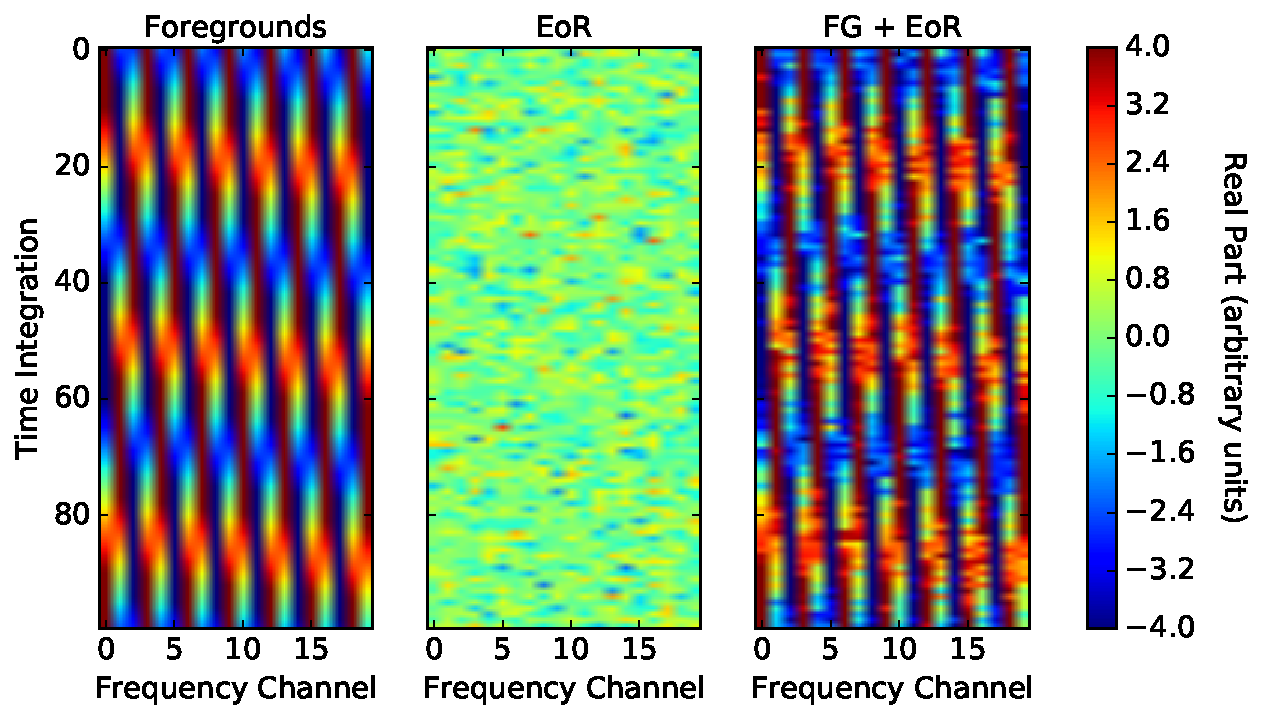
\includegraphics[trim={0cm 0cm 0cm 0cm},clip,width=0.7\textwidth]{plots/toy_sigloss1.pdf}
	\caption{Our toy model dataset to which we apply different weighting schemes to in order to investigate signal loss. We model a mock foreground-only visibility with a sinusoid signal that varies smoothly in 
time and frequency. We model a mock visibility of an EoR signal as a random Gaussian signal. We add the two together to form $\textbf{x} = 
\textbf{x}_{\rm FG} + \textbf{x}_{\rm EoR}$. Real parts are shown here.}
	\label{fig:toy_sigloss1}
\end{figure}

%First, 
We compute the power spectrum of our toy model dataset $\textbf{x}$ using Equations \eqref{eq:qhat} and \eqref{eq:phat}, with $\textbf{R} \equiv \widehat{\textbf{C}}^{-1}$.  Figure \ref{fig:toy_sigloss12} shows the estimated covariances of our toy model datasets along with the $\widehat{\textbf{C}}^{-1}$ weighted data. The foreground sinusoid is clearly visible in $\widehat{\textbf{C}}_{\rm FG}$.  The power spectrum result is shown in green in the left plot of Figure \ref{fig:toy_sigloss3}. Also plotted in the figure are the uniform-weighted ($\textbf{R} \equiv \textbf{I}$) power spectrum of the individual components $\textbf{x}_{\rm FG}$ (blue) and $\textbf{x}_{\rm EoR}$ (red). As shown, our $\widehat{\textbf{C}}^{-1}$ weighted result successfully suppresses foregrounds,
%For our toy model, the successful suppression of the foreground mode is 
demonstrated in Figure \ref{fig:toy_sigloss3} by the missing foreground peak in the weighted power spectrum estimate (green).  It is also evident that our result fails to recover the EoR signal --- it exhibits the correct shape, but the amplitude level is slightly low.  It is this behavior which we describe as signal loss.

\begin{figure}
	\centering
	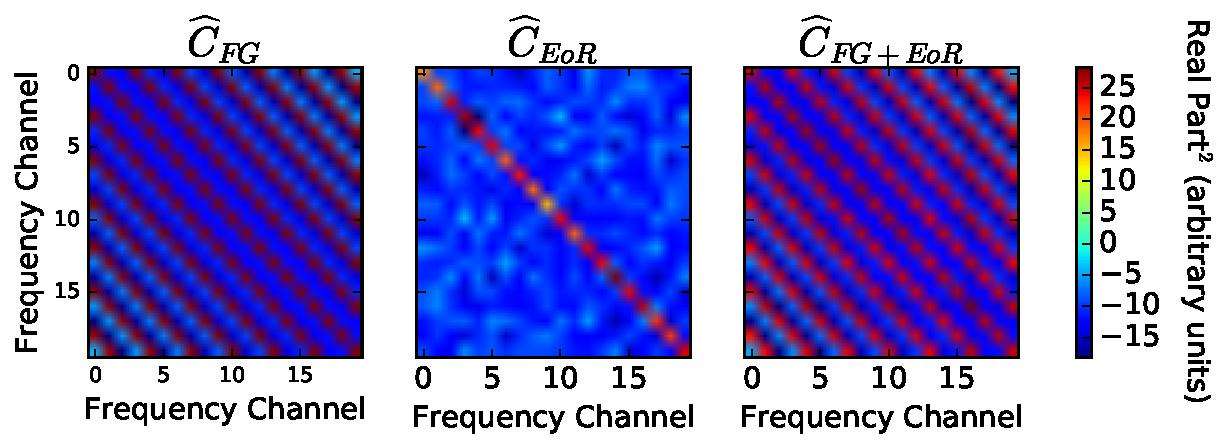
\includegraphics[trim={0cm 0cm 0cm 0cm},clip,width=0.7\textwidth]{plots/toy_sigloss12.pdf}
	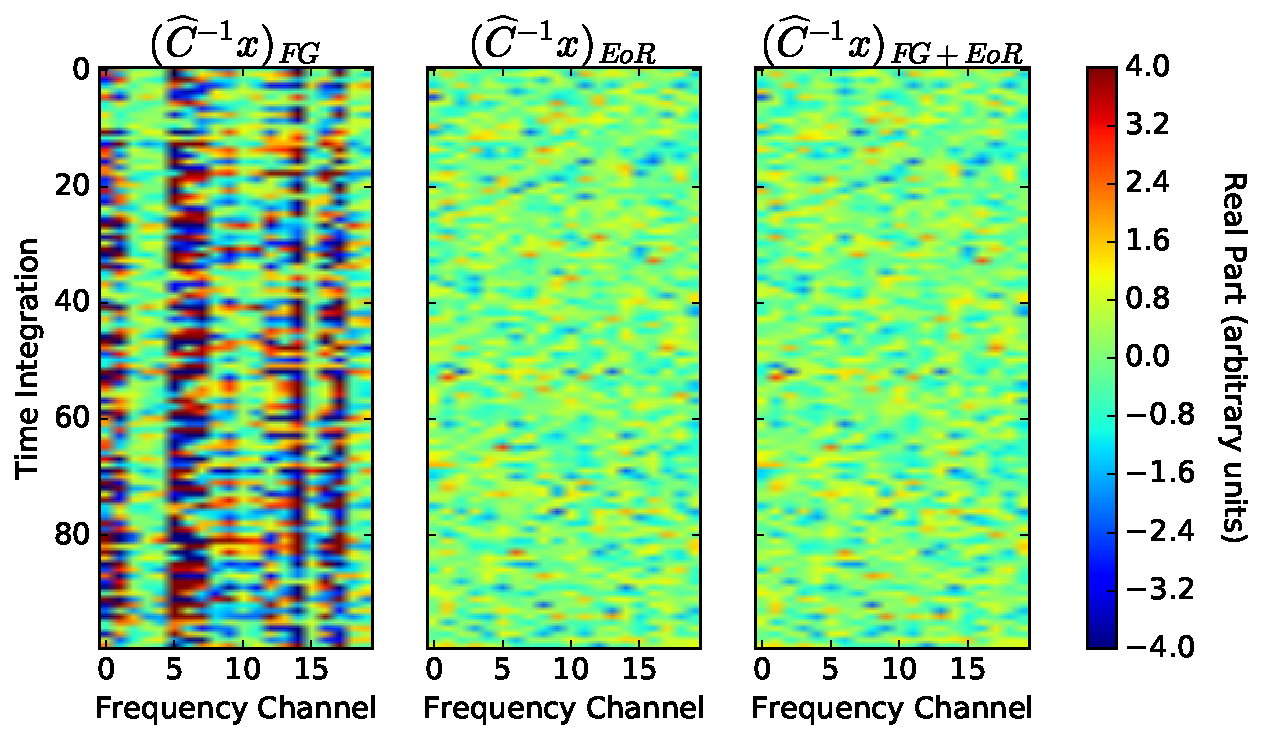
\includegraphics[trim={0cm 0cm 0cm 0cm},clip,width=0.7\textwidth]{plots/toy_sigloss13.pdf}
	\caption{The estimated covariance matrices (top row) and inverse covariance-weighted data (bottom row) for FG only (left), EoR only 
(middle), and FG + EoR (right). Real parts are shown here.}
	\label{fig:toy_sigloss12}
\end{figure}

\begin{figure*}
	\centering
	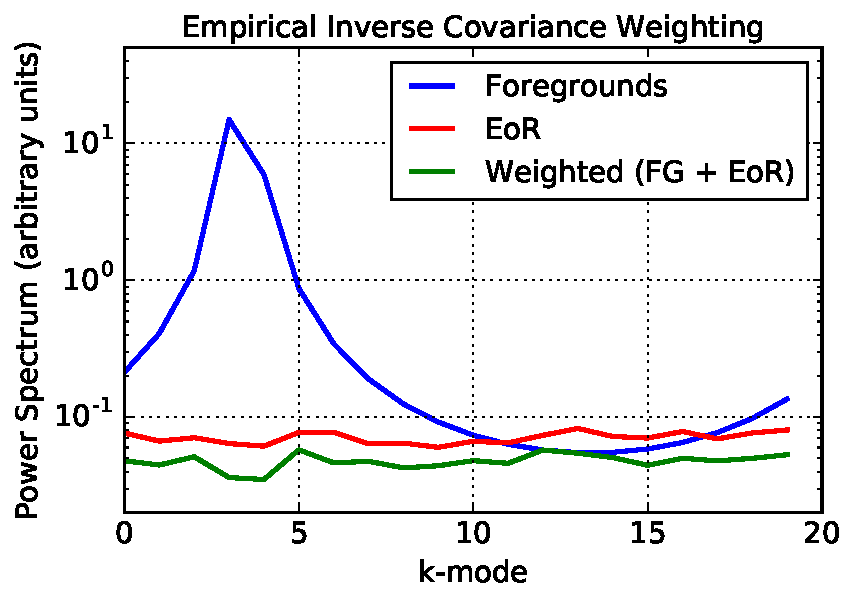
\includegraphics[trim={0cm 0cm 0cm 0cm},clip,height=0.33\textwidth]{plots/toy_sigloss3.pdf}
	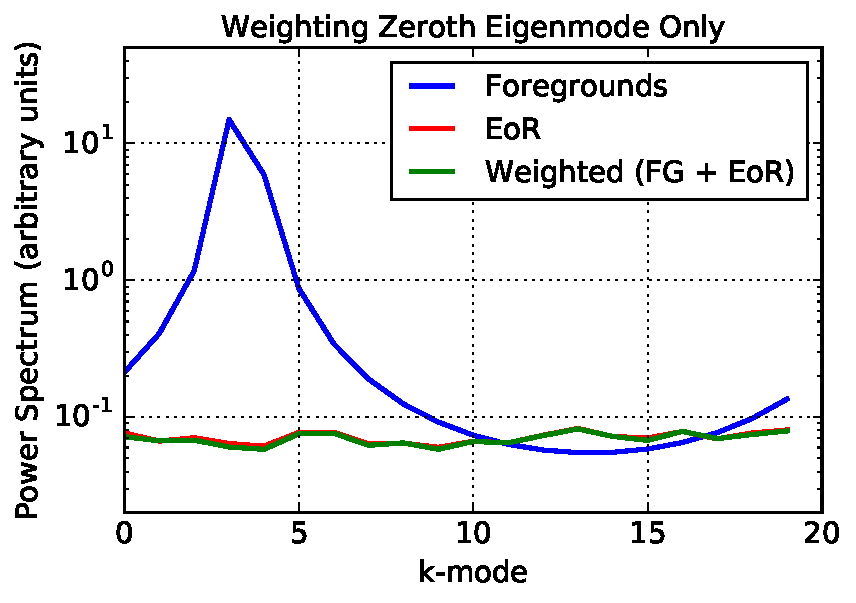
\includegraphics[trim={0cm 0cm 0cm 0cm},clip,height=0.33\textwidth]{plots/toy_sigloss4.pdf}
	\caption{Resulting power spectrum estimates for the toy model simulation described in Chapter \ref{sec:toymodel} --- foregrounds only (blue), EoR only (red), and the weighted FG + EoR dataset (green). The power spectrum of the foregrounds peaks at a $k$-mode based on the frequency of the sinusoid used to create the mock FG signal. In the two panels, we compare using empirically estimated inverse covariance weighting where $\textbf{C}$ is derived from the data (left), and projecting out the zeroth eigenmode only (right). In the former case, signal loss arises from the coupling of the eigenmodes of $\widehat{\textbf{C}}$ to the data. 
% JEA - redundant
%For an empirically estimated $\widehat{\textbf{C}}$, 
%its eigenvalues differ from those of the true covariance, where 
%the coupling between EoR-dominated eigenmodes and the data can lead to loss.
%Hence, 
There is negligible signal loss when all eigenmodes besides the foreground one are no longer correlated with the data.
%assigning identical weights to all eigenmodes except the first, 
%constructing a covariance proportional to the identity and the outer product of the sinusoid eigenmode, since we are only down-weighting the FG-dominated mode in this case.
}
	\label{fig:toy_sigloss3}
\end{figure*}

As discussed in Chapter \ref{sec:QE}, this behavior is {\it not} expected in the case that we were to use a true $\textbf{C}^{-1}$ weighting.  Rather, we would obtain the behavior shown in the toy model in Chapter \ref{sec:icw_appendix}\footnote{Note that there the true covariance matrix is also the sum of a diagonal portion describing the signal, and a single mode describing the contaminant (similar to Figure \ref{fig:toy_sigloss12}).}, with suppression of the foreground mode resulting in 
a nearly unbiased estimate of the power spectrum. The key difference is that since $\widehat{\textbf{C}}$ is estimated from the data, its eigenvectors and eigenvalues are strongly coupled to the particular data realization that was used to compute it, and this coupling leads to loss.

For the case of an eigenmode which can be safely assumed to be predominantly a foreground, its presence in the true covariance matrix will result in the desired suppression via a kind of projection; whether or not it is strongly correlated with the the actual data vector is irrelevant.  However, in the case of an empirically estimated covariance matrix, the eigenmodes of $\widehat{\textbf{C}}_{\rm EoR}$ will both be incorrect and can be correlated with the data. If these incorrect eigenmodes are not correlated with the data, it will lead to non-minimum variance estimates but will not produce the suppression of the power spectrum amplitude as seen in the left plot of Figure \ref{fig:toy_sigloss3}. As shown mathematically in Chapter \ref{sec:sigloss_appendix}, however, if $\widehat{\mathbf{C}}_{\rm EoR}$ $\textit{is}$ correlated with the data vector $\mathbf{x}$, there is a kind of projection of power in the {\it non}-foreground modes from the resulting power spectrum estimate, thus producing an estimate that is biased low.  In short, {\it if the covariance is computed from the data itself, it carries the risk of overfitting information in the data and introducing a multiplicative bias (per $k$) to estimates of the signal.} 

%For a toy model mathematical derivation of signal loss arising from a data-estimated covariance matrix, see Appendix \ref{sec:sigloss_appendix}. Here we will describe the origin of this signal loss intuitively.

%% JEA - I don't think the eigenspectrum really helps, but at some point we probably want to show it ...
%To begin to understand the lossy behavior of this result, we can closely study our estimated covariance eigenspectrum, shown in Figure \ref{fig:toy_sigloss2}. Since it is estimated from our data, its eigenspectrum differs from the eigenspectrum of the true covariance $\textbf{C}$, and this difference has important consequences on our result. 
%
%An eigenspectrum ranks the eigenvalues of a matrix from highest to lowest and can be thought of as a spectrum of weights that are given to each spectral mode in the data. In other words, the eigenvalues encode the strength of different shapes in the dataset. The eigenspectrum of the identity matrix $\textbf{I}$ is flat (all $1$'s) because it gives equal weighting to all modes. In our application, covariance matrices tend to have sloped eigenspectra, meaning that modes are given different weights in QE power spectrum estimation. 
%% JEA - I think this is actually NOT true - see the toy model as an example.  The size of the eigenvalues isn't what determines that the undesired mode is downweighted and the others left alone.  I haven't computed the eigenvalues explicitly, but down-weighting of m occurs regardless of the relative size of s and u.
%The modes with the highest eigenvalues are down-weighted the most. 

%\begin{figure}
%	\centering
%	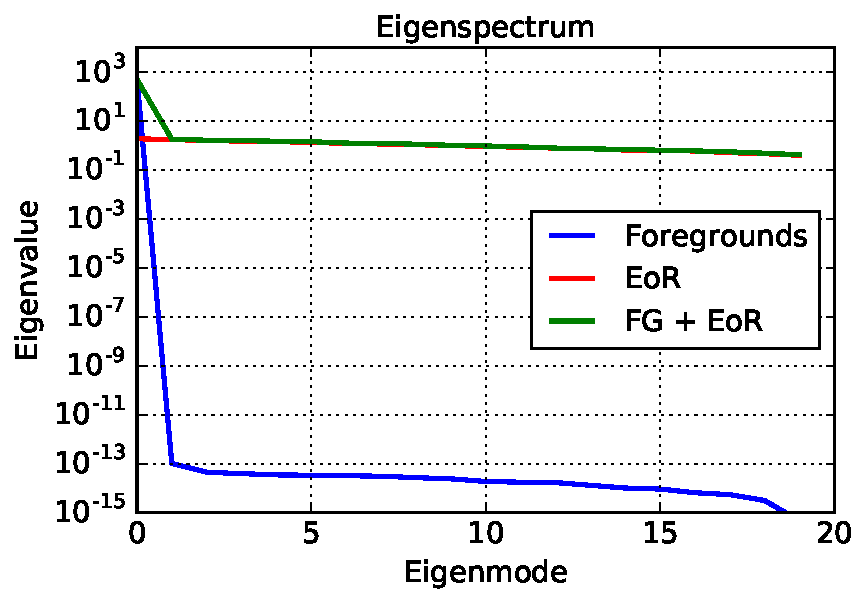
\includegraphics[trim={0cm 0cm 0cm 0cm},clip,width=\columnwidth]{plots/toy_sigloss2.pdf}
%	\caption{Eigenspectrum of $\widehat{\textbf{C}}_{\rm FG}$ (blue), $\widehat{\textbf{C}}_{\rm EoR}$ (red), and $\widehat{\textbf{C}}_{\rm FG+EoR}$ 
%(green). The eigenspectrum of $\widehat{\textbf{C}}_{\rm FG}$ peaks at the zeroth eigenmode, due to the presence of only one sinusoid. These empirically estimated covariance matrices have eigenspectra that are different from that of the true $\textbf{C}$. Specifically, these eigenmodes have the risk of being down-weighted more significantly than they should be because they are coupled to the data in a way that produces loss.}
%	\label{fig:toy_sigloss2}
%\end{figure}

%We show the {\it eigenspectrum} (the eigenvalues of the matrix in descending order) of this toy model in Figure \ref{fig:toy_sigloss2}.  In this case,
%For example, 
%the largest-valued eigenmode of $\widehat{\textbf{C}}$ (highest eigenvalue) describes the sinusoid foreground mode in the toy model (the peak in Figure \ref{fig:toy_sigloss3}). 
% 


%In general, the highest-valued eigenmodes of $\widehat{\textbf{C}}$ typically (but not always) describe bright foregrounds --- the most prominent shapes in a dataset. For these FG-dominated modes, where foregrounds outshine the EoR signal, down-weighting is beneficial. In some sense, we desire signal loss in this regime, if by `signal' we mean `foregrounds.' In this case it is beneficial for these eigenmodes to be coupled to the data in a way that produces loss. 



%If the true covariance matrix $\textbf{C}$ of our data was known, then every single eigenvalue and eigenvector of $\textbf{C}$ would be 
%representative of real fluctuations in the data. However, when using an estimated $\widehat{\textbf{C}}$ that is derived from one 
%particular data realization, its eigenvalues and eigenvectors may differ from the truth. Said differently, shapes that may not exist (or exist rarely) in a true covariance may appear stronger in the estimated covariance. Hence, they will be down-weighted 
%more than they should be.



The danger of an empirically estimated covariance matrix comes mostly from not being able to describe the EoR-dominated eigenmodes of $\textbf{C}$ accurately, for which the EoR signal is brighter than foregrounds. In such a case, the coupling between these modes to the data realization leads to the overfitting and subtraction of the EoR signal. More specifically, the coupling between the estimated covariance and the data is anti-correlated in nature (which is explained in more detail in Chapters \ref{sec:sigloss_appendix} and \ref{sec:siglossmethod}), which leads to loss. Mis-estimating $\textbf{C}$ for EoR-dominated eigenmodes is therefore more harmful than for FG-dominated modes, and since the lowest-valued eigenmodes of an eigenspectrum are typically EoR-dominated, using this part of the spectrum for weighting is most dangerous.

Armed with this information,
%Using what we've learned about the eigenspectrum, 
we can tweak the covariance in a simple way to suppress foregrounds and yield minimal signal loss. Recall that our toy model foreground 
% JEA - modes need not be sinusoids; the point is that there is one outer product describing this in the covariance
%is a sinusoid, so it 
can be perfectly described by a single eigenmode. Using the full dataset's (foreground plus EoR signal) empirical covariance, we can 
project out the zeroth eigenmode and 
%then flatten the rest of the spectrum to have eigenvalues of 1, thereby down-weighting the foreground-dominated mode more than the rest of the modes. Hence, we are changing the EoR-dominating part of the spectrum to be less coupled to the data, limiting the amount of overfitting that can happen for those modes (i.e., only allowing overfitting to occur for the first mode).
then take the remaining covariance to be the identity matrix.  
This decouples the covariance from the data for the EoR modes.  The resulting power spectrum estimate for this case is shown in the right plot of Figure \ref{fig:toy_sigloss3}. 
In this case we recover the EoR signal, demonstrating that if we can disentangle the foreground-dominated modes and EoR-dominated modes, we can suppress
% down-weight them 
foregrounds with negligible signal loss. 

Altering $\widehat{\textbf{C}}$ as such is one specific example of a regularization method for this toy model, in which we are changing $\widehat{\textbf{C}}$ in a way that reduces its coupling to the data realization. There are several other simple ways to regularize $\widehat{\textbf{C}}$, and we will discuss some in Chapter 
\ref{sec:otherweight}.

\subsection{Effect of Fringe-Rate Filtering}
\label{sec:toymodel_frf}

We have shown how signal loss can arise due to the coupling of EoR-dominated eigenmodes to the data. We will next show how this effect is exacerbated by reducing the total number of independent samples in a dataset. 

A fringe-rate filter is an analysis technique designed to maximize sensitivity by integrating in time (\citealt{parsons_et_al2016}). Rather than a traditional box-car average in time, a time domain filter can be designed to up-weight temporal modes consistent with the sidereal motion on the sky, while down-weighting modes that are noise-like. 

Because fringe-rate filtering is analogous to averaging in time, it comes at the cost of reducing the total number of independent samples in the data. With fewer independent modes, it becomes more difficult for the empirical covariance to estimate the true covariance matrix of the fringe-rate filtered data. We can quantify this effect by evaluating a convergence metric $\varepsilon(\Chat)$ for the empirical covariance, which we define as

% JEA - Death to eigenspectra!
%The resulting eigenspectrum as compared to the green curve (FG + EoR) in Figure \ref{fig:toy_sigloss2} is shown in Figure \ref{fig:toy_sigloss15}. 

\begin{equation}
\label{eq:converge}
\varepsilon (\Chat) \equiv \sqrt{\frac{\sum_{ij} (\widehat{C}_{ij} - {C}_{ij})^2}{\sum_{ij} {C}_{ij}^2}},
\end{equation}
where $\C$ is the true covariance matrix. To compute this metric, we draw different numbers of realizations (different draws of Gaussian noise) of our toy model EoR measurement, $\textbf{x}_{\rm EoR}$, and take their ensemble average. We then compare this to the ``true" covariance, which in our simulation is set to be the empirical covariance after a large number ($500$) of realizations. As shown in Figure \ref{fig:toy_sigloss16}, we perform this computation for a range of total independent ensemble realizations (horizontal axis) and number of independent samples in the data following time-averaging, or ``fringe-rate filtering" (different colors). With more independent time samples (i.e., more realizations) in the data, one converges to the true fringe-rate filtered covariance more quickly. 

The situation here with using a finite number of time samples to estimate our covariance is analogous to a problem faced in galaxy surveys, where the non-linear covariance 
of the matter power spectrum is estimated using a large --- but finite --- number of expensive simulations. There, the limited 
number of independent simulations results in inaccuracies in estimated covariance matrices 
\citep{dodelson_schneider2013,taylor_joachimi_etal2014}, which in turn result in biases in the final parameter constraints 
\citep{hartlap_et_al2007}. In our case, the empirically estimated covariances are used for estimating the power spectrum, and 
as we discussed in the previous section (and will argue more thoroughly in Chapters \ref{sec:sigloss_appendix} and \ref{sec:siglossmethod}), couplings between these covariances and the data can lead to power spectrum estimates that are biased 
\emph{low}---which is precisely signal loss. In future work, it will be fruitful to investigate whether advanced techniques from the 
galaxy survey literature for estimating accurate covariance matrices can be successfully adapted for $21\,\textrm{cm}$ 
cosmology. These techniques include the imposition of sparsity priors \citep{padmanabhan_et_al2016}, the fitting of 
theoretically motivated parametric forms \citep{pearson_samushia2016}, covariance tapering \citep{paz_sanchez2015}, 
marginalization over the true covariance \citep{sellentin_heavens2016}, and shrinkage methods 
\citep{pope_szapudi2008,joachimi_2017}.

%Just as important as the eigenvalues are the eigenvectors of our empirical covariances. 
The overall convergence of the covariance is important, but also noteworthy is the fact that different eigenvectors converge to their true forms at different rates. This is illustrated by Figure \ref{fig:toy_sigloss17}, which shows the convergence of eigenvectors in an empirical estimate of a covariance matrix. For this particular toy model, we construct a covariance whose true form combines the same mock foreground from the previous toy models with an EoR component that is modeled as a diagonal matrix with eigenvalues spanning one order of magnitude (more specifically, we construct the EoR covariance as a diagonal matrix in the Fourier domain, where the signal is expected to be uncorrelated; its Fourier transform is then the true covariance of the EoR in the frequency domain, or $\textbf{C}_{\rm EoR}$). For different numbers of realizations, we draw random EoR signals that are consistent with $\textbf{C}_{\rm EoR}$, add them to the mock foreground data, and compute the combined empirical covariance by averaging over the realizations. The eigenvectors of this empirical covariance are then compared to the true eigenvectors $\textbf{v}$, where we use as a convergence metric $\varepsilon(\widehat{\textbf{v}})$, defined as:
\begin{equation}
\label{eq:converge_eig}
\varepsilon (\widehat{\textbf{v}}) \equiv \sqrt{\sum_{i}^{N_{f}}|\textbf{v}-\widehat{\textbf{v}}|_{i}^2},
\end{equation}
where $N_{f}$ is the number of frequencies ($20$) in the mock data. The eigenmode convergence curves in Figure \ref{fig:toy_sigloss17} are ranked ordered by eigenvalue, such that ``Eigenmode \#0" illustrates the convergence of the eigenvector with the largest eigenvalue, ``Eigenmode \#1" for the second largest eigenvalue, and so on. We see that the zeroth eigenmode --- the mode describing the foreground signal --- is quickest to converge.

Our numerical test reveals that the convergence rates of empirical eigenvectors is related to the sample variance in our empirical estimate. In general, computing an empirical covariance from a finite ensemble average means that the empirical eigenmodes have sample variances. Consider first a limiting case where all eigenvalues are equal. In such a scenario, any linear combination of eigenvectors is also an eigenvector, and thus there is no sensible way to define the convergence of eigenvectors. In our current test, aside from the zeroth mode, the eigenvalues have similar values but are not precisely equal. Hence, there is a well-defined set of eigenvectors to converge to. However, due to the sample variance of our empirical covariance estimate, there may be accidental degeneracies between modes, where some modes are mixing and swapping with others. Therefore, the steeper an eigenspectrum, the easier it is for the eigenmodes to decouple from each other and approach their true forms. A particularly drastic example of this can be seen in the behavior of mode $0$ (the foreground mode), whose eigenvalue differs enough from the others that it is able to converge reasonably quickly despite substantial sample variance in our empirical covariance estimate. To break degeneracies in the remaining modes, however, requires many more realizations.

While the connection between the rate of convergence of an empirical eigenvector with the sample variance of an eigenspectrum is interesting, it is also important to note that regardless of convergence rate, any mode that is coupled to the data is susceptible to signal loss. The true eigenvectors are not correlated with the data realizations; thus, if our empirical eigenvectors are converged fully, there will not be any signal loss. However, an unconverged eigenvector estimate will retain some memory of the data realizations used in its generation, leading to signal loss.

In the toy models throughout Chapter \ref{sec:SiglossOverview}, we exploit the fact that the strongest eigenmode (highest eigenvalue mode) is dominated by foregrounds in order to purposely incur signal loss for that mode. Even for the case of real PAPER data (Chapter \ref{c.PSA64}), we make the assumption that the strongest eigenmodes are likely the most contaminated by foregrounds. However, in general, foregrounds need not be restricted to the strongest eigenmodes, and as we have seen, it is really the degeneracies between modes that determines how quickly they converge, and hence how much signal loss can result.

%One sees that the highest-valued eigenmodes converge to their true eigenvectors more quickly. With only a small number of realizations, these empirically estimated modes already retain little correlation with the specific realizations of data that were used to form the empirical covariance. As we will see in the next section, using only these eigenmodes, which are less coupled to data realizations, minimizes signal loss. In contrast, the lower-valued eigenmodes retain more memory of the data realizations, which leads to correlations that induce signal loss. 
% JEA - this is redundant
%Said differently, a steep covariance eigenspectrum can be especially dangerous because the eigenmodes that converge the slowest are typically also EoR-dominated and are therefore susceptible to the most loss.  %\acl{Think about whether we need to do the Fourier space version as well.}

% JEA - death to eigenspectra!
%\begin{figure}
%	\centering
%	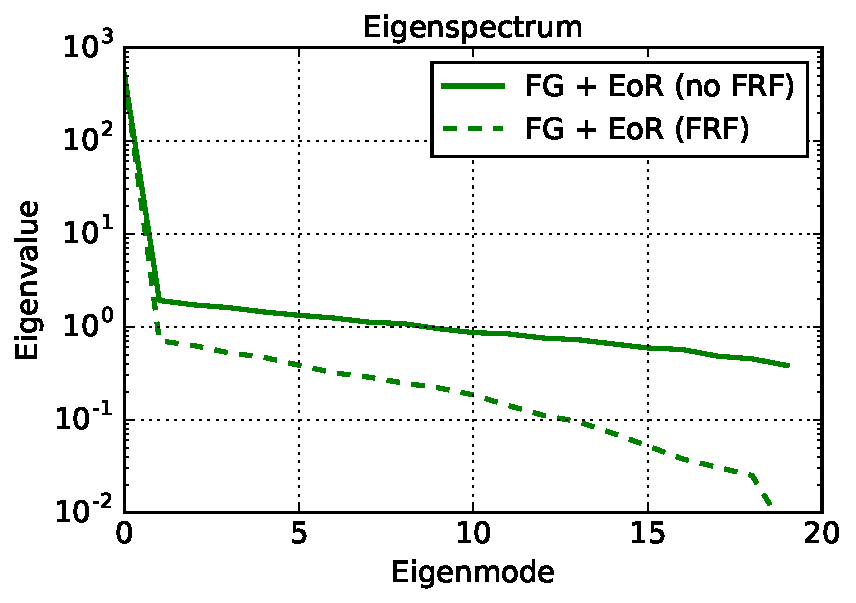
\includegraphics[trim={0cm 0cm 0cm 0cm},clip,height=0.31\textwidth]{plots/toy_sigloss15.pdf}
%	\caption{Eigenspectrum of $\widehat{\textbf{C}}_{\rm FG+EoR}$, in the case of no fringe-rate filtering (solid green) and with fringe-rate filtering (dashed green). The dashed, steep eigenspectrum has a greater risk of signal loss because its lowest-valued eigenmodes are both more strongly coupled to the data (than those of the solid eigenspectrum) and, in this example, are also EoR-dominated.}
%	\label{fig:toy_sigloss15}
%\end{figure}

\begin{figure}
	\centering
	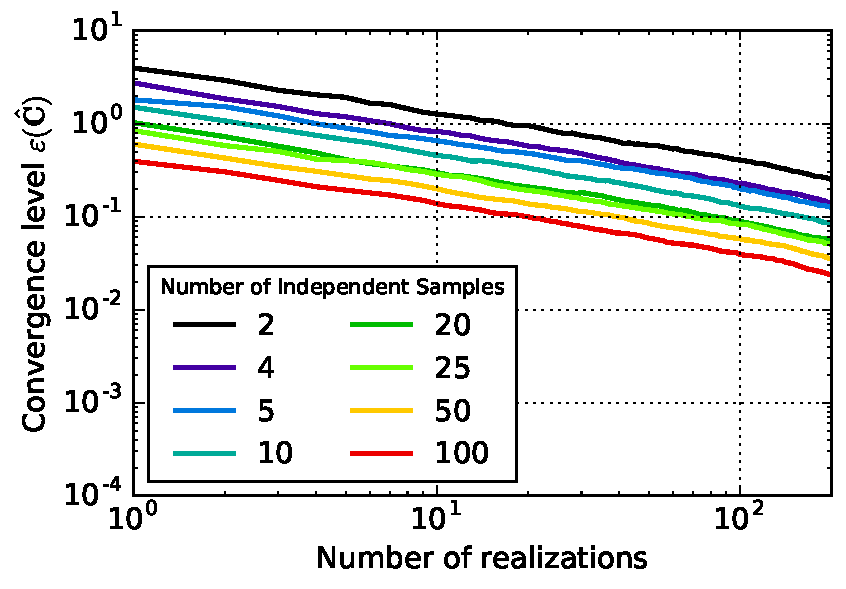
\includegraphics[width=0.55\textwidth]{plots/toy_sigloss16.pdf}
	\caption{The convergence level, as defined by Equation \eqref{eq:converge}, of empirically estimated covariances of mock EoR signals with different numbers of independent samples. In red, the mock EoR signal is comprised entirely of independent samples (100 of them). Subsequent colors show time-averaged signals. As the number of realizations increases, we see that the empirical covariances approach the true covariances. With more independent samples, the quicker an empirical covariance converges (i.e., the quicker it decouples from the data), and the less signal loss we would expect to result.}
	\label{fig:toy_sigloss16}
\end{figure}

\begin{figure}
	\centering
	\includegraphics[width=0.7\textwidth]{plots/toy_sigloss17.pdf}
	\caption{The convergence level, as defined by Equation \eqref{eq:converge_eig}, of empirically estimated eigenvectors for different numbers of mock data realizations. The colors span from the 0th eigenmode (has the highest eigenvalue) to the 19th eigenmode (has the lowest eigenvalue), where they are ordered by eigenvalue in descending order. This figure shows that the zeroth eigenmode converges the quickest, implying that eigenvectors with eigenvalues that are substantially different than the rest (the FG-dominated mode has a much higher eigenvalue than the EoR modes) are able to converge to the true eigenvectors the quickest. On the other hand, eigenmodes $1$-$19$ have similar eigenvalues and are slower to converge because of degeneracies between them.}
	\label{fig:toy_sigloss17}
\end{figure}

\begin{figure}
	\centering
	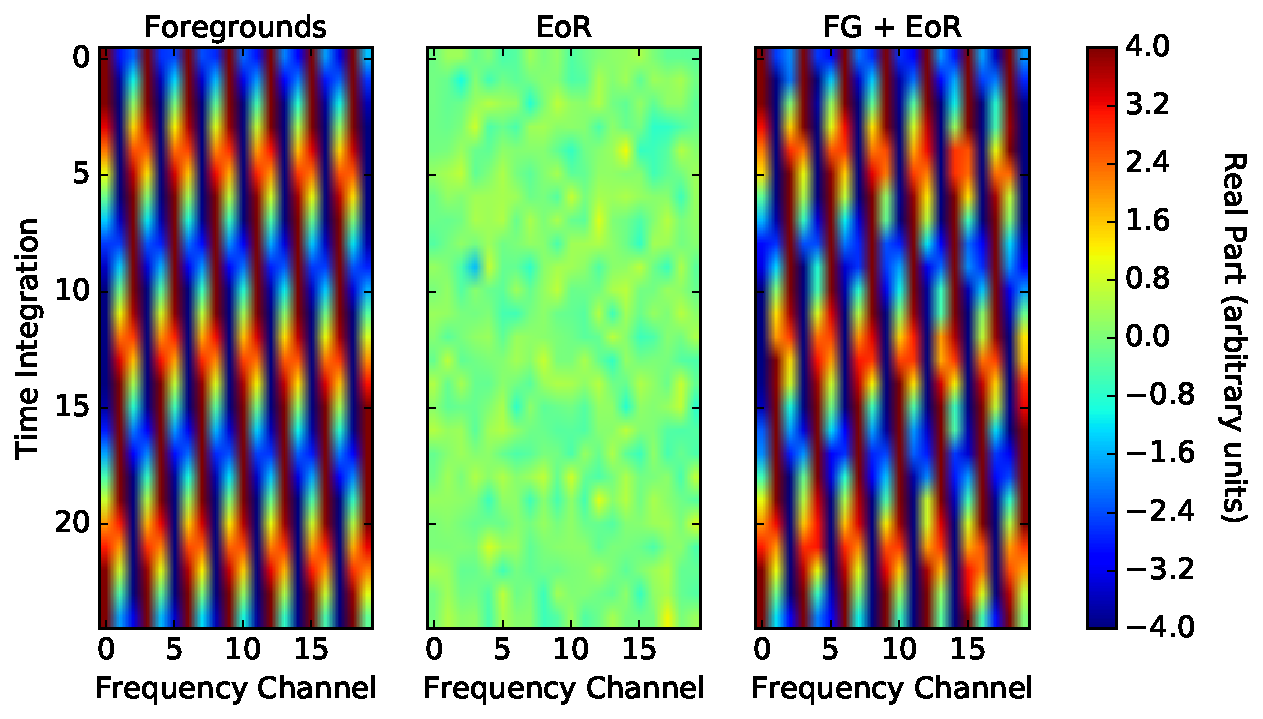
\includegraphics[width=0.7\textwidth]{plots/toy_sigloss5.pdf}
	\caption{Our ``fringe-rate filtered" (time-averaged) toy model dataset. We average every four samples together, 
yielding $25$ independent samples in time. Real parts are shown here.}
	\label{fig:toy_sigloss5}
\end{figure}


With Figures \ref{fig:toy_sigloss16} and \ref{fig:toy_sigloss17} establishing the connection between convergence rates (of empirical covariances and eigenvectors) and number of realizations, we now turn back to our original toy model used in Chapter \ref{sec:toymodel}, which is comprised of a mock foreground and mock EoR signal. We mimic a fringe-rate filter by averaging every four time integrations of our toy model dataset together, yielding $25$ independent samples in time (Figure \ref{fig:toy_sigloss5}). We choose these numbers so that the total number of independent samples is similar to the number of frequency channels --- hence our matrices will be full rank. We use this ``fringe-rate filtered" mock data for the remainder of Chapter \ref{sec:SiglossOverview}.
%\footnote{If instead we average every $20$ samples together, yielding only $5$ independent samples in time, we are left with a rank deficient covariance matrix. In this case... \cc{fill in}}

The power spectrum results for this model are shown in Figure \ref{fig:toy_sigloss7}, and as 
expected there is a much larger amount of signal loss for this time-averaged dataset since we do a worse job estimating the true covariance. In addition, as a result of having fewer independent samples, we obtain an estimate with more scatter. This is evident by noticing that the 
green curve in Figure \ref{fig:toy_sigloss7} fails to trace the shape of the uniform-weighted EoR power spectrum (red). 

Using our toy model, we have seen that a sensitivity-driven analysis technique like fringe-rate filtering has trade-offs of signal 
loss and noisier estimates when using data-estimated covariance matrices. Longer integrations increase sensitivity but reduce 
the number of independent samples, resulting in 
eigenmodes correlated with the data
% JEA - it's not that they are wrong, but that they are correlated
%poorly characterized, steep eigenspectra 
that can overfit signal greatly. We 
note that a fringe-rate filter does have a range of benefits, many described in \citet{parsons_et_al2016}, so it can still be 
advantageous to use one despite the trade-offs.

\begin{figure}
	\centering
	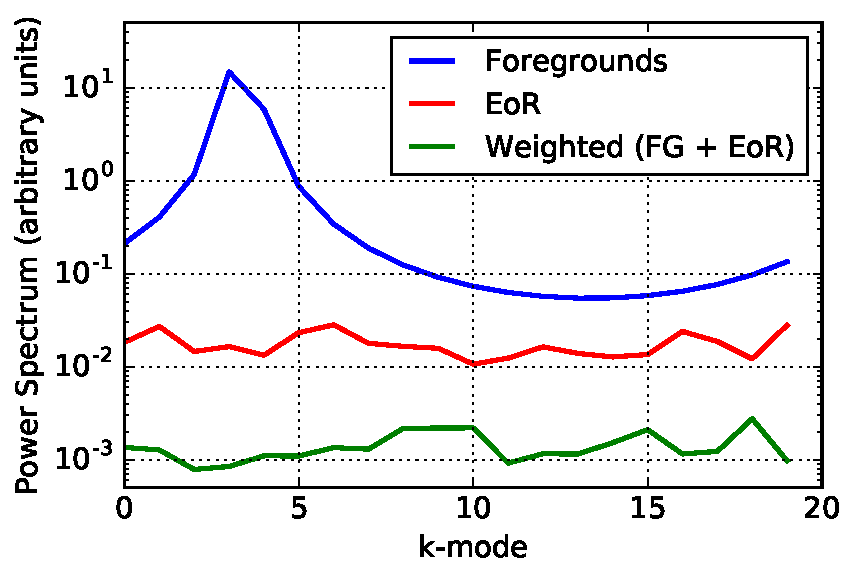
\includegraphics[trim={0cm 0cm 0cm 0cm},clip,width=0.7\textwidth]{plots/toy_sigloss7.pdf}
	\caption{Resulting power spectrum estimate for the ``fringe-rate filtered" (time-averaged) toy model simulation --- foregrounds only (blue), 
EoR only (red), and the weighted FG + EoR dataset (green). We use empirically estimated inverse covariance weighting where $\textbf{C}$ is 
computed from the data. There is a larger amount of signal loss than for the non-averaged data, a consequence of weighting by eigenmodes that are more strongly coupled to the data due to there being fewer independent modes in the data.}
	\label{fig:toy_sigloss7}
\end{figure}

\subsection{Other Weighting Options}
\label{sec:otherweight}

In Chapter \ref{sec:toymodel} we showed one example of how altering $\widehat{\textbf{C}}$ can 
make the difference between nearly zero and some signal loss. We will now use our toy model to describe several other ways to tailor $\widehat{\textbf{C}}$ 
in order to minimize signal loss. We choose four independent regularization methods to highlight in this section, which have 
been chosen due to their simplicity in implementation and straightforward interpretations. We illustrate the resulting power 
spectra for the different cases in Figure \ref{fig:toy_sigloss8}.
% and \ref{fig:toy_sigloss14}. 
These examples are not meant to be taken as suggested analysis methods but rather as illustrative cases. 

As a first test, we model the covariance matrix of EoR as a proof of concept that if perfect models are known, signal loss can be 
avoided. We know that our simulated EoR signal should have a covariance matrix that mimics the identity matrix, with its 
variance encoded along the diagonal. We model $\textbf{C}_{\rm EoR}$ as such (i.e., the identity), instead of computing it based on $\textbf{x}
_{\rm EoR}$ itself. Next, we add $\textbf{C}_{\rm EoR} + \widehat{\textbf{C}}_{\rm FG}$ (where $\widehat{\textbf{C}}_{\rm FG} = \langle\textbf{x}_{\rm FG}
\textbf{x}_{\rm FG}^{\dagger}\rangle_{t}$) to obtain a final $\widehat{\textbf{C}}_{\rm reg}$ (regularized empirical covariance matrix) to use in weighting. In Figure \ref{fig:toy_sigloss8} (upper 
left), we see that there is negligible signal loss. This is because by modeling $\textbf{C}_{\rm EoR}$, we avoid overfitting EoR fluctuations in the data that our model doesn't know about (but, an empirically derived $\widehat{\textbf{C}}_{\rm EoR}$ would know about the fluctuations). 
%This is also shown by comparing the (steeper) green and (flatter) red curves in Figure \ref{fig:toy_sigloss14}. 
In practice such a weighting option is not feasible, as it is difficult to model $\textbf{C}_{\rm EoR}$, and $\widehat{\textbf{C}}_{\rm FG}$ is unknown because we do not know how to separate out the foregrounds from the EoR in our data.

\begin{figure*}
	\centering
	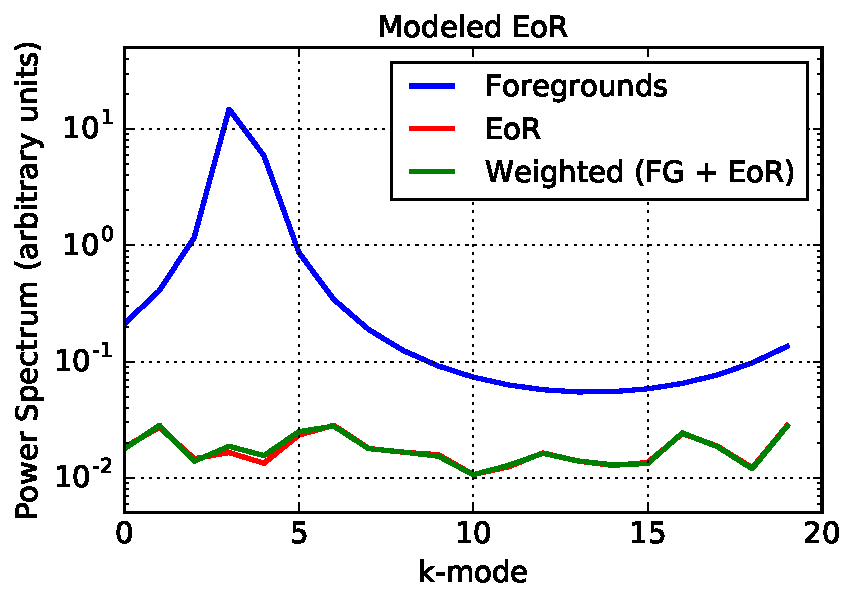
\includegraphics[trim={0cm 0cm 0cm 0cm},clip,height=0.33\textwidth]{plots/toy_sigloss10.pdf}
	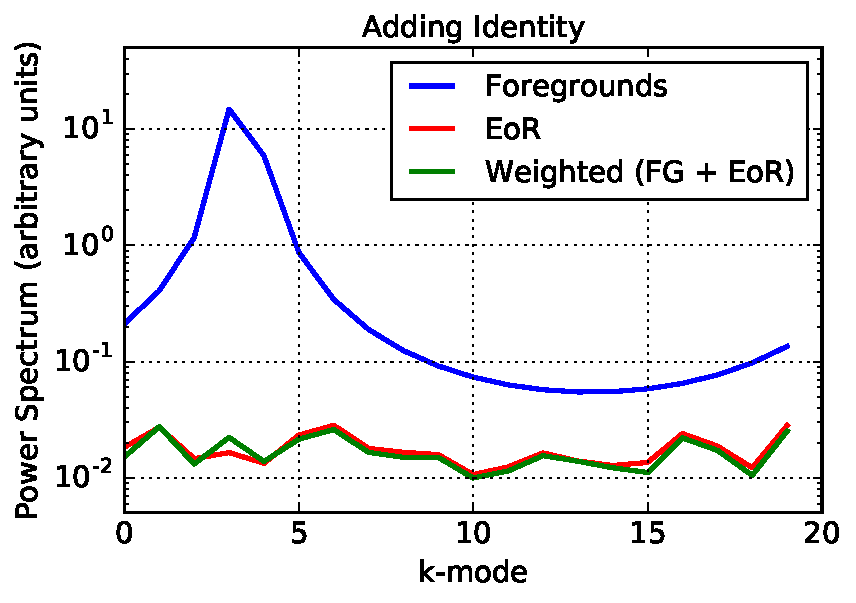
\includegraphics[trim={0cm 0cm 0cm 0cm},clip,height=0.33\textwidth]{plots/toy_sigloss8.pdf}
	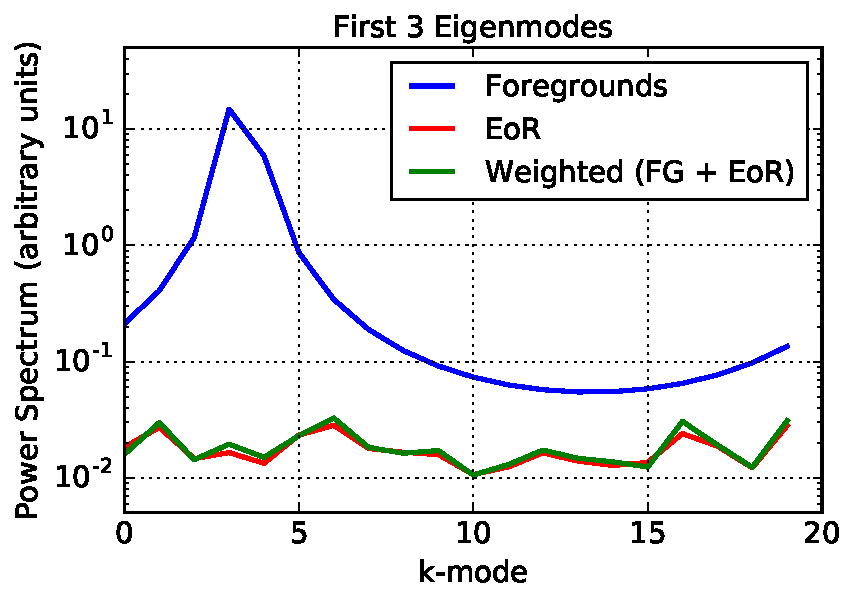
\includegraphics[trim={0cm 0cm 0cm 0cm},clip,height=0.33\textwidth]{plots/toy_sigloss9.pdf}
	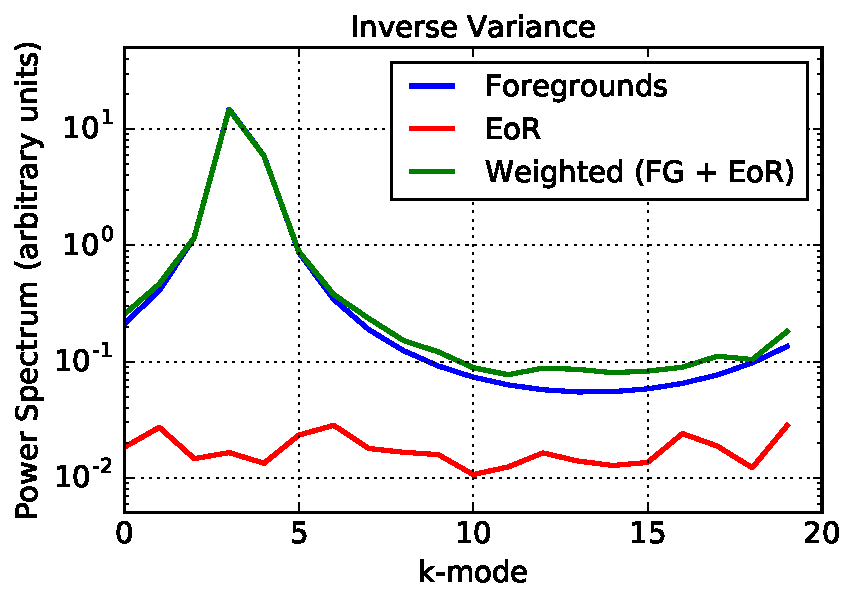
\includegraphics[trim={0cm 0cm 0cm 0cm},clip,height=0.33\textwidth]{plots/toy_sigloss11.pdf}
	\caption{Resulting power spectra estimates for our ``fringe-rate filtered" (time-averaged) toy model simulation --- foregrounds only (blue), EoR only (red), and the weighted FG + EoR dataset (green). We show four alternate weighting options that each minimize signal loss, including modeling the covariance matrix of EoR (upper left), regularizing $\widehat{\textbf{C}}$ by adding an identity matrix to it (upper right), using only the first three eigenmodes of $\widehat{\textbf{C}}$ (lower left), and keeping only the diagonal elements of $\widehat{\textbf{C}}$ (lower right). The first case (upper left) is not feasible in practice since we do not know $\textbf{C}_{\rm FG}$ and $\textbf{C}_{\rm EoR}$ like we do in the toy model.}
	\label{fig:toy_sigloss8}
\end{figure*}

%\begin{figure}
%	\centering
%	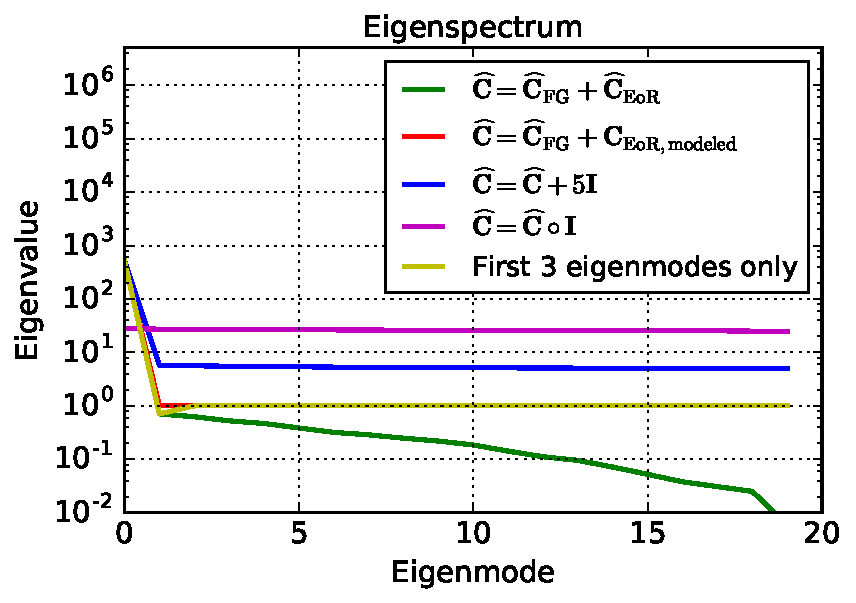
\includegraphics[trim={0cm 0cm 0cm 0cm},clip,width=\columnwidth]{plots/toy_sigloss14.pdf}
%	\caption{We compare the eigenspectrum of an empirically calculated $\widehat{\textbf{C}}$ (green) to that of four alternate 
%weighting options, including modeling the covariance matrix of EoR (red), regularizing $\widehat{\textbf{C}}$ by adding an identity 
%matrix to it (blue), using only the first three eigenmodes of $\widehat{\textbf{C}}$ (yellow), and multiplying an identity matrix with $
%\widehat{\textbf{C}}$ (magenta). All eigenspectra (except the green) are relatively flat and don't exhibit signal loss. All were 
%computed for the `fringe-rate filtered' (time-averaged) toy model case presented in Chapter \ref{sec:toymodel_frf}.}
%	\label{fig:toy_sigloss14}
%\end{figure}
%
The second panel (top right) in Figure \ref{fig:toy_sigloss8} uses a regularization method of setting $\widehat{\textbf{C}}_{\rm reg} \equiv 
\widehat{\textbf{C}} + \gamma\textbf{I}$, where $\gamma = 5$ (an arbitrary strength 
of $\textbf{I}$ for the purpose of this toy model). By adding the identity matrix, element-wise, we are weighting the diagonal 
elements of the estimated covariance matrix more heavily than those off-diagonal. Since the identity component does not know anything about the data realization, it alters the covariance to be less coupled to the data and there is no loss. %Although there is negligible signal loss using this regularization, the small green peak at the fourth $k$-mode represents residual foregrounds that still exist since the shapes encoded in the off-diagonal frequency correlations of the covariance matrix were deemed not as prominent as the diagonal elements using this weighting scheme. 

The third panel (bottom left) in Figure \ref{fig:toy_sigloss8} minimizes signal loss by only using the first three eigenmodes of the estimated covariance. Recalling that our toy model foregrounds can be described entirely by the zeroth eigenmode, this 
method intentionally projects out the highest-valued modes only by replacing all but the three highest weights in the 
eigenspectrum with $1$'s (equal weights). Again, avoiding the overfitting of EoR-dominated modes which are coupled to the data results in negligible signal loss. While this case is illuminating for the toy model, in practice it is not obvious which eigenmodes are foreground or EoR dominated (and they could be mixed as well), so determining which subset of modes to down-weight is not trivial. We experiment with this idea using PAPER data in Chapter \ref{sec:Weight}.

The last regularization scheme we are highlighting here is setting $\widehat{\textbf{C}}_{\rm reg} \equiv \widehat{\textbf{C}} \circ \textbf{I}$ (element-wise multiplication), or inverse variance weighting (i.e., keeping only the diagonal elements of $\widehat{\textbf{C}}$). In the bottom right 
panel of Figure \ref{fig:toy_sigloss8}, we see that this method does not down-weight the foregrounds at all --- this regularization altered $\widehat{\textbf{C}}$ in a way where it is no longer coupled to \textit{any} of the empirically estimated eigenmodes, including the FG-dominated one. To understand this, we recall that our foregrounds are spread out in frequency and therefore have non-negligible frequency-frequency correlations. Multiplying by 
the identity matrix, element-wise, results in a diagonal matrix, meaning we do not have any correlation information. Because of this, we do a poor job 
suppressing the foreground. But because we decoupled the whole eigenspectrum from the data, we also avoid signal loss. Although this method did not successfully recover the EoR signal for this particular simulation, it is important that we show that there 
are many options for estimating a covariance matrix, and some may down-weight certain eigenmodes more effectively than others based on the spectral nature 
of the components in a dataset. 
%One may imagine a situation where a particular systematic is contained to an isolated 
%frequency (such as radio frequency interference or crosstalk). In such a case, preserving only the diagonal elements of $
%\widehat{\textbf{C}}$ would be an effective way of removing this contamination. 

In summary, we have shown how signal loss is caused by weighting a dataset by itself, and in particular how estimated covariances can overfit EoR modes when they are coupled to data and not converged to their true forms. We have also seen that there are trade-offs between a chosen weighting method, its foreground-removal effectiveness, the number of independent samples in a dataset, and the amount of resulting signal loss. 

\section{Signal Loss Mathematical Framework}
\label{sec:SiglossMath}

In Chapter \ref{sec:QE}, we argued that the optimal quadratic estimator method has the effect of projecting out foreground modes that have a different covariance structure than the EoR signal. And in Chapter \ref{sec:toymodel}, we saw that \textit{empirical} inverse covariance weighting can lead to loss via a multiplicative bias to estimates of the signal. To support these arguments, we now present two mathematical frameworks in which we use toy models in order to illustrate these conclusions analytically. 

\subsection{A Toy Model for Inverse Covariance Weighting}
\label{sec:icw_appendix}

%AAAXXX

In this section, we focus on the optimal quadratic estimator, Equation \eqref{eq:OQE}, and mathematically illustrate its role in estimating the power spectrum of EoR. While there exists detailed literature about quadratic estimators in general (e.g., \citealt{liu_tegmark2011}; \citealt{trott_et_al2012}; \citealt{liu_et_al2014b}; \citealt{dillon_et_al2014}), here we focus on two simple cases in order to outline one situation where the estimator successfully suppresses contamination and one where it does not. By describing these two cases, we hope to clarify and motivate the desire to use OQE while also understanding its limitations.

In our toy model, we specifically choose toy models where the data covariance is diagonal, as indeed we expect the EoR signal to be. We assume we have $N$ data points $\Delta_i$ which are the sum of a desired signal $\sigma_i$ and an undesired contaminant $\upsilon_i$
\begin{equation}
\Delta_i = \sigma_i + \upsilon_i
\end{equation}
with 
\begin{equation}
\langle \sigma_i \rangle = 0; \; \langle \sigma^2_i \rangle = s; \; {\rm and}~\langle \bm{\sigma \sigma}^T \rangle = s \mathbf{I}_{N \times N} \equiv \mathbf{S},
\end{equation}
where we wish to estimate $s$.  The contaminant in this first case has a similar structure (as the EoR) for its covariance, and is assumed uncorrelated with the signal
\begin{equation}
\label{eq:IdealToyModelCovariance}
\langle \upsilon_i \rangle = 0; \; 
\langle \upsilon^2_i \rangle = u; \; 
\langle \bm{\upsilon \upsilon}^T \rangle = u \mathbf{I}_{N \times N} \equiv \mathbf{U}; {\rm and}~ 
\langle \sigma_i \upsilon_j \rangle = 0.
\end{equation}
With the covariance matrix given by $\C = \mathbf{S} + \mathbf{U}$, the estimator for $s$ using only the quadratic part of Equation \ref{eq:OQE} is
\begin{equation}
\label{eq:IdealToyModelEstimator}
\hat{s} = \frac{ \bm{\Delta^T \Delta}}{N} 
\end{equation}
and its expectation is
\begin{equation}
\langle \hat{s} \rangle = s + u.
\end{equation}
Thus, {\it when the covariance structure of the contaminant is identical to the signal} ($\PDeriv{\mathbf{S}}{s} = \PDeriv{\mathbf{U}}{u} =  \PDeriv{\C}{s}$), the information available to the quadratic portion of the estimator to distinguish between the two is degenerate, and knowledge only of $\C$ and $\PDeriv{\C}{s}$ is inadequate.  In order to obtain an unbiased estimate of $s$, one must also use knowledge of $\mathbf{U}$.  Indeed, computing the linear bias from Equation \eqref{eq:OQELinear}, one finds $b = u$.   

Now consider a case, chosen to be very similar to the toy model in \ref{sec:toymodel},  in which the data again have an additive contaminant, now given by
\begin{equation}
\Delta_i = \sigma_i + \upsilon m_i
\end{equation}
where the properties of $\sigma_i$ are as before, but now $\upsilon$ is a random variable and $m_i$ is a fixed function of $i$ with
\begin{equation}
\langle \upsilon \rangle = 0; \;
\langle \upsilon^2 \rangle = u; \; 
 \langle \bm{\upsilon \upsilon}^T \rangle = u \mathbf{m m}^T \equiv \mathbf{U}; \;
 \mathbf{m}^T \mathbf{m} = 1; \; {\rm and}~ 
\langle \sigma_i \upsilon \rangle = 0.
\end{equation}
Here $\mathbf{m}$ represents a mode which is correlated across many data points (i.e., we are assuming $\mathbf{U}$ need {\it not} be diagonal), with amplitude given by  $\upsilon$.  The normalization of $\mathbf{m}$ is a matter of convention, and can be absorbed in the variance $u$; the choice above will be convenient for understanding the limiting case $u \gg s$.

We can calculate the quadratic portion of the estimator explicitly by using the Sherman-Morrison identity to invert the covariance matrix.  Defining
\begin{equation}
\xi \equiv \frac{u/s}{1+u/s},
\end{equation} 
we have
\begin{equation}
\invC  =   \frac{1}{s} \left(\I - \xi \mathbf{m m}^T \right)
\end{equation}
and
\begin{equation}
\hat{s} = 
%\half {\F}^{-1} \left(\bm \Delta^T \invC \PDeriv{\C}{s}  \invC \bm \Delta \right) = 
\frac{ \bm \Delta^T  (\I +  (\xi^2 - 2 \xi)  \mathbf{m m}^T)  \bm \Delta}{N + \xi^2 - 2 \xi} 
\end{equation}
with expectation
\begin{equation}
\langle \hat{s} \rangle = 
s + \frac{1 - 2 \xi + \xi^2}{N + - 2 \xi + \xi^2} u. 
\end{equation}
It is worth observing immediately that there is no multiplicative bias on $s$, and that the additive bias is strictly $< u/N$.

An instructive limit is $u \gg s$, $\xi \to 1$, in which case the virtue of weighting by $\invC$ becomes clearer, as it becomes
\begin{equation}
\invC  = \frac{1}{s} \left(\I - \mathbf{m m}^T \right)
\end{equation}
where $\I - \mathbf{m m}^T$ is the projection operator, projecting out $\mathbf{m}$ from any vector it acts on, and further, the linear bias tends to 0 as $\xi \to 1$ (i.e., the projection is ``perfect'' and not ``undone'' by the Fisher matrix normalization).

This is the ideal case for the inverse covariance weighting performed in the PAPER analysis, where removal of contamination with a known covariance can be suppressed by a kind of projection of the offending modes.  But even in this case, it is worth pointing out that the estimator still has a linear bias for finite $u$.  We have also assumed that the contaminating mode $\mathbf{m}$ is known perfectly; the next section takes up the case where the modes are estimated from the data.

\color{black}

%\appendix
\subsection{A Toy Model for Signal Loss}
\label{sec:sigloss_appendix}

In this section, we examine a toy model for signal loss. Our goal is to derive an analytic formula for power spectrum signal loss. While this model does not apply generally to all the scenarios presented in this work, it provides some analytic intuition for how the coupling between data and an empirical covariance can result in signal loss.

The minimum-variance quadratic estimator $\widehat{P}^\alpha$ for the $\alpha$th bandpower of the power spectrum is given by 
\begin{equation}
\widehat{P}^\alpha = \frac{1} {2 \F^{\alpha \alpha} }\x^t \C^{-1} \Q^{\alpha} \C^{-1} \x,
\end{equation}
where
\begin{equation}
F^{\alpha \alpha} \equiv \frac{1}{2} \textrm{tr} \left( \C^{-1} \Q^\alpha \C^{-1} \Q^\alpha \right)
\end{equation}
is the $\alpha$th diagonal element of the Fisher matrix. For this section only, with no loss of generality, we assume that the data $\textbf{x}$ are real. We also assume for simplicity that $\mathbf{x}$ is the data from a single instant in time, so that it is of length $N_f$, where $N_f$ is the number of frequency channels.

In our case, we do not have \emph{a priori} knowledge of the covariance matrix. Thus, we deviate from the true minimum-variance quadratic estimator and replace $\C$ with $\Chat$, its data-derived approximation. Our estimator then becomes
\begin{equation}
\label{eq:phatloss}
\widehat{P}^\alpha_\textrm{loss} = \frac{1} {2 \widehat{\F}^{\alpha \alpha} }\x^t \Chat^{-1} \Q^{\alpha} \Chat^{-1} \x,
\end{equation}
where
\begin{equation}
\widehat{F}^{\alpha \alpha} \equiv \frac{1}{2} \textrm{tr} \left( \Chat^{-1} \Q^\alpha \Chat^{-1} \Q^\alpha \right),
\end{equation}
with the label ``loss" to foreshadow the fact that this will be an estimator with signal loss (i.e., a multiplicative bias of less than unity). We will now provide an explicit demonstration of this by modeling the estimated covariance as
\begin{equation}
\label{eq:ChatDef}
\Chat = (1-\eta) \C + \eta \x \x^t,
\end{equation}
where $\eta$ is a parameter quantifying our success at estimating the true covariance matrix. If $\eta = 0$, our covariance estimate has perfectly modeled the true covariance and $\Chat = \C$. On the other hand, if $\eta =1$, then our covariance estimate is based purely on the one realization of the covariance that is our actual data, and we would expect a high level of overfitting and signal loss.

Our strategy for computing the signal loss will be to insert Equation \eqref{eq:ChatDef} into Equation \eqref{eq:phatloss} and to express the resulting estimator $\widehat{P}^\alpha_\textrm{loss}$ in terms of $\widehat{P}^\alpha$. We begin by expressing $\Chat^{-1}$ in terms of $\C^{-1}$ using the Woodbury identity so that
\begin{equation}
\Chat^{-1} = \frac{\C^{-1}}{1-\eta} \left[ \I - \frac{\eta \x \x^t \C^{-1}}{1+ \eta (g-1)}\right],
\end{equation}
where we have defined $g \equiv \x^t \C^{-1} \x$. Inserting this into our Fisher estimate we have
\begin{equation}
\widehat{F}^{\alpha \alpha} = \frac{F^{\alpha \alpha}}{(1-\eta)^2} \left[ 1 -\frac{\eta }{1+ \eta (g-1)} \frac{h^{\alpha \alpha}}{F^{\alpha \alpha}} + \frac{1}{2} \left( \frac{\eta }{1+ \eta (g-1)} \right)^2 \frac{(h^{\alpha})^2}{F^{\alpha \alpha}}\right],
\end{equation}
where $h^\alpha \equiv \x^t \C^{-1} \Q^\alpha \C^{-1} \x $ and $h^{\alpha \alpha} \equiv \x^t \C^{-1} \Q^\alpha \C^{-1} \Q^\alpha \C^{-1}\x $. Note that $g$, $h^\alpha$, and $h^{\alpha \alpha}$ are all random variables, since they depend on $\x$. Inserting these expressions into our estimator gives
\begin{equation}
\label{eq:phatlossexpanded}
\widehat{P}^\alpha_\textrm{loss} = \frac{1}{2} \frac{h^\alpha}{F^{\alpha \alpha}} \left[ 1 - \frac{\eta g}{1+ \eta (g-1)}\right]^2  \left[ 1 -\frac{\eta }{1+ \eta (g-1)} \frac{h^{\alpha \alpha}}{F^{\alpha \alpha}} + \frac{1}{2} \left( \frac{\eta }{1+ \eta (g-1)} \right)^2 \frac{(h^\alpha)^2}{F^{\alpha \alpha}}\right]^{-1}.
\end{equation}
Both for the purposes of analytical tractability and to provide intuition, we expand this expression to leading 
order in $\eta$. This approximates the limiting case where the covariance $\Chat$ is close to the ideal and the 
lossy covariance is a small perturbation.  The result is
\begin{equation}
\widehat{P}^\alpha_\textrm{loss} \approx \frac{1}{2} \frac{h^\alpha}{F^{\alpha \alpha}} \left[ 1 - \eta \left( g - \frac{h^{\alpha \alpha}}{F^{\alpha \alpha}}\right)\right].
\end{equation}
Taking the ensemble average of both sides and noting that the true power spectrum $P^\alpha$ is equal to $\langle h^\alpha \rangle / 2 F^{\alpha \alpha}$, we obtain
\begin{equation}
\langle \widehat{P}^\alpha_\textrm{loss} \rangle \approx (1- \eta N_f) P^\alpha + 4 \eta \frac{\rm{tr} (\C^{-1} \Q^\alpha \C^{-1} \Q^\alpha \C^{-1} \Q^\alpha )}{\left[ \rm{tr} (\C^{-1} \Q^\alpha \C^{-1} \Q^\alpha  ) \right]^2} \approx (1- \eta N_f) P^\alpha,
\end{equation}
where recall that $N_f$ is the length of $\x$, or the number of frequency channels. In the last step we dropped the final term, since it scales as $\eta P^\alpha$ (without the factor of $N$) and is therefore typically small compared to the terms that have been retained.

Recalling that $P^\alpha$ is the \emph{true} power spectrum, one sees that when the covariance in the optimal quadratic estimator is naively replaced by an empirical covariance, the resulting power spectrum estimate is biased low, i.e., there is signal loss. This occurs because of couplings between $\widehat{\C}$ and $\x$, which formally means that what was originally a quadratic estimator is no longer quadratic, but contains higher-order correlations. This violates the assumptions implicit in the derivation of $F^{\alpha \alpha}$ as the normalization factor for converting unnormalized bandpowers $\frac{1}{2} \x^t \C^{-1} \Q^{\alpha} \C^{-1} \x$ into properly normalized power spectrum estimates, where the unnormalized bandpowers are assumed to be two-point (i.e., quadratic) statistics \citep{liu_tegmark2011}. The result is an improperly normalized---and thus lossy---power spectrum estimate.

\section{Error Estimation Toy Model}
\label{sec:ErrorOverview}

Our second major 21\,cm power spectrum theme is error estimation, as we desire robust methods for determining accurate 
confidence intervals for our measurements. Two popular ways of calculating errors on a power spectrum 
measurement are calculating the variance of power spectrum results, and computing a theoretical error estimate based on an instrument's 
system temperature and observational parameters. In a perfect world, both methods would match up. However, in practice the 
two do not always agree due to a number of factors, including possible non-Gaussianities in the noise properties of our instruments and possible systematics in the data.

A third option which acts as a middle ground between purely theoretical and purely empirical errors is using Gaussian error. This involves the assumption of Gaussianity, but allows the variance of the power spectrum estimator to be written as a function of the two-point estimator, or covariance. One could empirically calculate the covariance and then propagate it into an analytic expression to compute the errors, making this method fall somewhere between being fully empirical and fully modeled (see \citet{das_et_al2011a} for an example of its implementation). 

For PAPER's analysis, we choose a data-driven method of error estimation that does not rely on assumptions of Gaussianity. Namely, we compute error bars that have been derived from the inherent 
variance of our measurements. A common technique used to do this is bootstrapping. For pedagogical purposes, we first define the technique of 
bootstrapping and then illustrate one of its pitfalls through a toy model.

Bootstrapping uses sampling with replacement to estimate a posterior distribution. For example, measurements (like power 
spectra) can be made from different samples of data. Each of these measurements is a different realization drawn from some underlying distribution, and realizations are correlated with each other to a degree set by the fraction of sampled points that are held in common 
between them. Through the process of re-sampling and averaging along different axes of a dataset, such as along baselines or times, we can estimate error bars for 
our results which represent the underlying distribution of values that are allowed by our measurements (\citealt{efron_tibshirani1994}; \citealt{andrae2010}).

Suppose we have $N$ different measurements targeting the same quantity (for example, $N$ power spectrum measurements). 
Bootstrapping means that we form $N_{\rm boot}$ (often a large number) bootstraps, where each bootstrap is a random selection 
of the $N$ measurements. Bootstraps each have dimensions of $N$, and the values populated into each bootstrap are drawn 
from the original set of measurements with replacement (i.e., every $n^{th}$ slot in $N$ is filled randomly for each bootstrap). Next we take 
the mean of each bootstrap to collapse it from an array of length $N$ to a single number (we are interested in the mean statistic 
here, but any function of interest can be applied to each bootstrap as long as it's the same function for each one). The error (on 
the mean) is then computed as the standard deviation across all bootstraps. 

We must be careful in distinguishing $N_{\rm boot}$, the number of bootstraps, from $N$, the number of samples, or elements, or 
values, that comprise a bootstrap. In the toy models presented in this section, $N_{\rm boot}$ is typically large, and the standard 
deviation across bootstraps (the error we are computing) converges for large $N_{\rm boot}$. Typically $N$ is a straightforward value to set that just depends on the experiment. However, we will illustrate one case in which it is not simply the number of samples along the axis that is being re-sampled. More specifically, we will see that $N$ depends on sample independence and may not always be straightforward to approximate. 

For our toy model, suppose we have a Gaussian random signal dataset of length $N=1000$ and unity variance (zero mean). 
This could represent $1000$ power spectrum measurements, for which we are interested in its error. We predict that the error 
on the mean should obey $1/\sqrt{N}$, where $N$ is the number of samples.

We next form $500$ bootstraps ($N_{\rm boot} = 500$). To create each bootstrap, we draw $N$ samples, with replacement, of the 
original data, and take the mean over the $N$ samples. The standard deviation over the $500$ bootstraps gives an error 
estimate for our dataset. This error is indicated by the gray star in Figure \ref{fig:toy_error1} and matches our theoretical 
prediction (green).

\begin{figure}
	\centering
	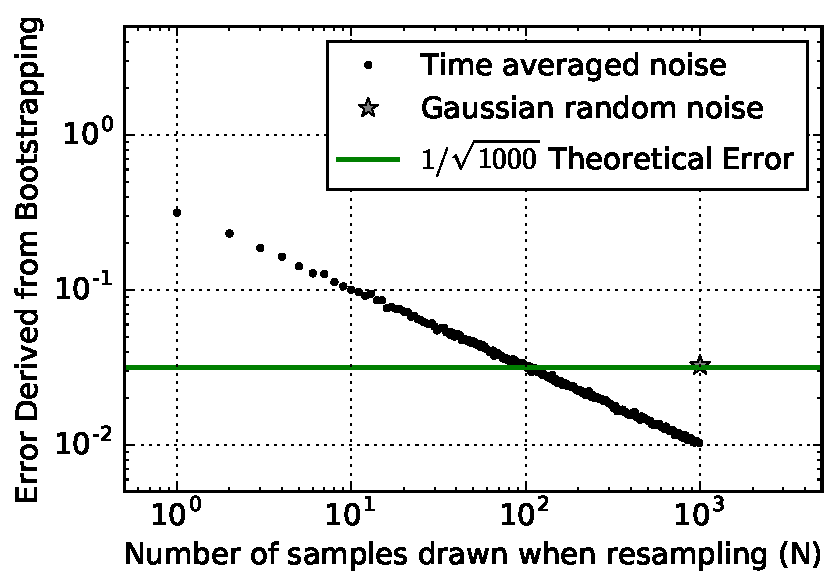
\includegraphics[trim={0cm 0cm 0cm 0cm},width=0.7\textwidth]{plots/toy_error1.pdf}
	\caption{Error estimation from bootstrapping as a function of the number of elements drawn per bootstrap when 
sampling with replacement. The star represents the standard deviation of $N_{\rm boot}=500$ bootstraps, each created by drawing $1000$ 
elements (with replacement) from a length $1000$ array of a Gaussian random signal. The black points correspond to time-averaged data (correlated data) which has $100$ independent samples. They illustrate how errors can be under-estimated if 
drawing more elements than there are independent samples in the data. The estimated errors match up with the theoretical 
prediction only at $N=100$.}
	\label{fig:toy_error1}
\end{figure}

One major caveat of bootstrapping arises when working with correlated data. If, for example, a dataset has many repeated 
values inside it, this would be reflected in each bootstrap. The same value would be present multiple times within a bootstrap 
and also be present between bootstraps, purely because it has a more likely chance of being drawn if there are repeats of 
itself. Therefore, bootstrapping correlated data results in a smaller variation between bootstraps, and hence, under-estimates 
errors. The use of a fringe-rate filter, which averages data in time to increase sensitivity, is one example which leads to a 
reduction in the number of independent samples, creating a situation in which errors can be under-estimated. We will now show 
this effect using our toy model.

Going back to our toy model, we apply a sliding boxcar average to $10$ samples at a time, thus reducing the number of 
independent data samples to $N/10 = 100$. Bootstrapping this time-averaged noise, using the same method as described 
earlier (drawing $N=1000$ elements per bootstrap sample), under-estimates the error by a factor of $\sim3$ (black points in Figure \ref{fig:toy_error1}, at $N=1000$). This occurs 
because we are drawing more samples than independent ones available, and thus some samples are repeated multiple times 
in all bootstraps, leading to less variation between the bootstraps. In fact, the error derived from bootstrapping is a strong 
function of the number of elements that are drawn per bootstrap (Figure \ref{fig:toy_error1}, black points), and we can both 
under-estimate the error by drawing too many or over-estimate it by drawing too few. However, since we know that we have $100$ 
independent samples in this toy model, the error associated with drawing $N=100$ samples with replacement does match the theoretical prediction 
as expected (the black points cross the green line at $N=100$ in Figure \ref{fig:toy_error1}).

This example highlights the importance of understanding how analysis techniques (such as fringe-rate filtering) can affect a 
common statistical procedure like bootstrapping. Bootstrapping as a means of estimating power spectrum errors from real 
fringe-rate filtered data requires knowledge of the number of independent samples, which is not always a trivial task. For 
example, computing the effective number of independent samples of fringe-rate filtered data is not as simple as counting the 
number of averages performed. Down-sampling a time-averaged signal is straightforward using a boxcar average, but non-trivial with a more complicated convolution function that has long tails. Hence, we do not recommend bootstrapping unless the 
number of independent samples along the axis that is being re-sampled is well-determined. In Chapter \ref{sec:Boot}, we explain how we under-estimated errors in the \citetalias{ali_et_al2015} analysis of PAPER and how our bootstrapping procedure has now changed to avoid the over-sampling of correlated data. 

In summary, bootstrapping can be an effective and straightforward way to estimate errors of a dataset. However, we have 
illustrated a situation in which bootstrapping can lead to under-estimated errors and therefore under-estimated power spectrum limits. We have shown that 
bootstrapped error depends strongly on the number of elements drawn in a bootstrap sample. Estimated errors can drop to 
arbitrarily small values when the number of elements drawn exceeds the effective number of independent elements. 
%We have also shown a situation in which a bootstrapping method does not provide the most sensitive measurement possible. 
While bootstrapping is convenient because it provides a way to estimate errors from the data itself, one must assess whether certain 
analysis choices have compromised the method and whether a variation or an avoidance of traditional re-sampling could be preferred instead.

\section{Bias Toy Model}
\label{sec:BiasOverview} % make sure this is the same as original paper when put in

In a 21\,cm power spectrum, detections could be the EoR signal, but they could also 
%(and unfortunately more likely) 
be attributed to other sources of bias. Connecting a detection to EoR as opposed to noise or foreground bias is a key challenge of 
future 21\,cm data analyses \citep[e.g.][]{petrovic_and_oh2011}. In this section we will discuss possible sources of bias in a measurement, as well as techniques 
that can help mitigate their effects. We will also present a series of tests in a pedagogical fashion which we suggest be used to 
help evaluate deep limits and/or detections.

\subsection{Foreground and Noise Bias}
\label{sec:BiasTypes}

In Chapter \ref{sec:SiglossOverview}, we discussed signal loss as a form of multiplicative bias to estimates of the signal. Foregrounds are another type of bias, but an additive instead of a multiplicative one. Foreground bias is perhaps one of the main factors limiting 21\,cm results, as foreground signals lie $\sim4$-$5$ orders of 
magnitude above the cosmological signal. Though there are many techniques proposed for removing foregrounds (see e.g. \citealt{vedantham_et_al2012}; \citealt{chapman_et_al2012}; \citealt{parsons_et_al2012a}; \citealt{parsons_et_al2012b}; \citealt{dillon_et_al2013a}; \citealt{wang_et_al2013}; \citealt{parsons_et_al2014}; \citealt{liu_et_al2014a}; \citealt{wolz_et_al2014}; \citealt{liu_et_al2014b}; \citealt{dillon_et_al2015}; \citealt{pober_et_al2016a}; \citealt{trott_et_al2016}), most 
experiments currently remain limited by residuals rather than noise, especially at low $k$.

One common method to isolate and filter foregrounds is to exploit their behavior in $k$-space. For a particular 
baseline length, there is a maximum delay imposed on sources attached to the sky, which corresponds to the light-crossing time between two 
antennas in a baseline. For longer baselines, this value increases, producing what is known as ``the 
wedge"
\citep{datta_et_al2010, parsons_et_al2012b, vedantham_et_al2012, pober_et_al2013, thyagarajan_et_al2013, liu_et_al2014a, liu_et_al2014b, patil_et_al2017}. 
The wedge describes a region in $k$-space contaminated by smooth spectrum foregrounds, bounded by baseline length (which is proportional to $k_{\perp}$) and delay (which is 
proportional to $k_{\parallel}$). Properties of the wedge can be used to isolate and 
%remove 
avoid foregrounds, as done by \citetalias{ali_et_al2015}, 
\citet{parsons_et_al2014}, \citet{dillon_et_al2014}, \citet{dillon_et_al2015}, \citet{jacobs_et_al2015}, \citet{beardsley_et_al2016}, and \citet{trott_et_al2016}.

Although smooth-spectrum foregrounds preferentially show up at low delay, or low $k$-modes, their isolation within the wedge is not perfect. In deep measurements, power spectrum measurements at $k_{\parallel}$ values beyond 
the delay associated with the length of a baseline are often still contaminated at a low level. This leakage, particularly at low $k$'s, can be attributed to 
convolution kernels associated with Fourier-transforming visibilities into delay-space. In other words, smooth-spectrum 
foregrounds appear as $\delta$-functions in delay-space, convolved by the Fourier transform of the source spectrum, the signal chain, and the 
antenna response, all of which could smear out the foregrounds and cause leakage outside the wedge \citep[e.g.][]{ewall-wice_et_al2017, kerrigan_et_al2018}.

There are analysis techniques to mitigate the effects of foreground leakage and prevent information from low $k's$ from 
spreading to high $k$ values. For example, narrow window functions in delay-space can be used to minimize the leakage from a particular 
$k$ value into other ones (\citealt{liu_et_al2014b}). In other words, one can construct an estimator using QE that forces a 
window function to have a minimum response to low $k$ values. The window function used in \citetalias{ali_et_al2015} is constructed in such a way, 
specifically to prevent foregrounds that live at low $k's$ from contaminating higher $k$-modes (see Chapter \ref{sec:Bias}). 

Determining the source of positive non-EoR detections at higher $k$'s is more difficult. In previous power spectrum results, these detections have been explained as instrumental systematics, particularly time-variable cross talk, RFI, cable reflections, and calibration errors (\citetalias{ali_et_al2015}; \citealt{parsons_et_al2014}; \citealt{dillon_et_al2014}; \citealt{beardsley_et_al2016}; \citealt{patil_et_al2017}). In the next section, we will present some tests that can help distinguish these excesses from that of EoR. 

In addition to foreground bias, noise can also be responsible for positive power spectrum detections if thermal noise is 
multiplied by itself. Every 21\,cm visibility measurement contains thermal noise that is comprised of receiver and sky noise. 
We expect this noise to be independent between antennas and thus we can beat it down (increase sensitivity) by integrating 
longer, using more baselines, etc. However, the squaring of noise can occur when cross-multiplying visibilities, which is shown by 
the two copies of $\textbf{x}$ in Equation \eqref{eq:qhat}. If both copies of $\textbf{x}$ come from the same baseline and time, it 
can result in power spectrum measurements that are higher than those predicted by the thermal noise of the instrument. One 
way to avoid this type of noise bias is to avoid cross-multiplying data from the same baselines or days. This ensures that the 
two quantities that go into a measurement have separate noises that don't correlate with each other. We also note that if the noise level is known, this type of bias can be subtracted off, though this procedure is argued to be dangerous (\citealt{dillon_et_al2014}; \citealt{parsons_et_al2014}).

Another type of noise bias can stem from the spurious cross-coupling of signals between antennas. This excess is known as 
instrumental crosstalk and is an inadvertent correlation between two independent measurements via a coupled signal path. 
Crosstalk varies on a time-scale much slower than the typical fringe-rates of 
sources. Because it is slow-varying, crosstalk can be suppressed using time-averages or fringe-rate filters. However, there 
remains a possibility that power spectrum detections that aren't the cosmological signal are caused by residual, low-level crosstalk which survived any 
suppression techniques. 

\subsection{Jackknife Tests}
\label{sec:JackknifeOverview}

We now approach the difficult task of tracing excesses to foreground, noise, and EoR biases through a discussion of useful 
jackknife tests. Again, we first approach this topic pedagogically as an introduction to the related PAPER discussion in Chapter 
\ref{sec:Bias}. 

The jackknife is a resampling technique in which a statistic (i.e., power spectrum) is computed in subsets of the data (\citealt{quenouille1949}; \citealt{tukey1958}). These 
subsets are then compared to reveal systematics. In this section we define two main tests --- the null test and the traditional 
jackknife --- and explain how a power spectrum detection must pass each. We then highlight how these tests can be used to 
help distinguish between different sources of bias.
 
\begin{itemize}
\item \textbf{Null Test}: A null test is a type of jackknife test that removes the astronomical signal from data in order to 
investigate underlying systematics (see \citet{keating_et_al2016} for examples from intensity mapping that are closely related to our current application). For example, one can 
divide data into two subsets by separating odd and even Julian dates, or the first half of the observing season from the second. 
Subtracting the two removes signal that is common to both subsets, including foregrounds and the EoR signal. The resulting power 
spectrum should be consistent with thermal noise estimates; if it is not, it suggests the presence of a systematic that differs 
from one of the data subsets to the other (i.e., doesn't get subtracted perfectly). 
\item \textbf{Traditional Jackknife}: In a broader sense, it is important to perform many jackknife tests in order to instill 
confidence in a final result. A stable result must be steadfast throughout all jackknives no matter how the data is sliced. 
Jackknives can be taken along several different axes --- for example, one could start with a full dataset, and compute a new 
power spectrum every time as a day of data is removed, or a baseline is removed. This type of jackknife would reveal bias 
present only at certain LSTs (such as a foreground source), for example, or misbehaving baselines.
\end{itemize}

While the null test hunts for deviations from thermal noise and the jackknife tests for deviations in subsamples, they are both 
closely related. We can highlight the connection between the two using a toy model dataset.

Suppose we have four independent measurements made along two different axes. As an example, we construct $\textbf{x}_{1a}$, $\textbf{x}_{1b}$, $\textbf{x}_{2a}$, and $\textbf{x}_{2b}$, where the numbers symbolize two different days of data and the letters represent two different baselines. Each of the 
measurements have dimensions of $100$ time integrations and $20$ frequency channels. They each have separate thermal 
noises constructed as a Gaussian random signal for each, and identical EoR signals. 

To mimic the presence of a systematic, we add a toy sinusoid foreground, similar to the one used in 
Chapter \ref{sec:toymodel}, to only $\textbf{x}_{2a}$ and $\textbf{x}_{2b}$. This represents a foreground signal 
present in only the second day of data, but not the first. Mathematically, if  $\textbf{n}$ 
is noise, $\textbf{e}$ is the EoR signal, and $\textbf{f}$ is the foreground signal, the four measurements can be written as:

\begin{eqnarray}
\label{eq:bias1}
\textbf{x}_{1a} &=& \textbf{n}_{1a} + \textbf{e}  \\ 
\textbf{x}_{1b} &=& \textbf{n}_{1b} + \textbf{e}  \\ 
\textbf{x}_{2a} &=& \textbf{n}_{2a} + \textbf{e} + \textbf{f} \\ 
\textbf{x}_{2b} &=& \textbf{n}_{2b} + \textbf{e} + \textbf{f}.
\end{eqnarray} 

\noindent We now take a jackknife along the day-axis, forming separate power spectrum estimates for each day:

\begin{eqnarray}
\widehat{\textbf{P}}_{1} &\propto& \textbf{x}_{1a}\textbf{x}_{1b}^{\dagger} \\
\widehat{\textbf{P}}_{2} &\propto& \textbf{x}_{2a}\textbf{x}_{2b}^{\dagger}.
\end{eqnarray}

\begin{figure}
	\centering
	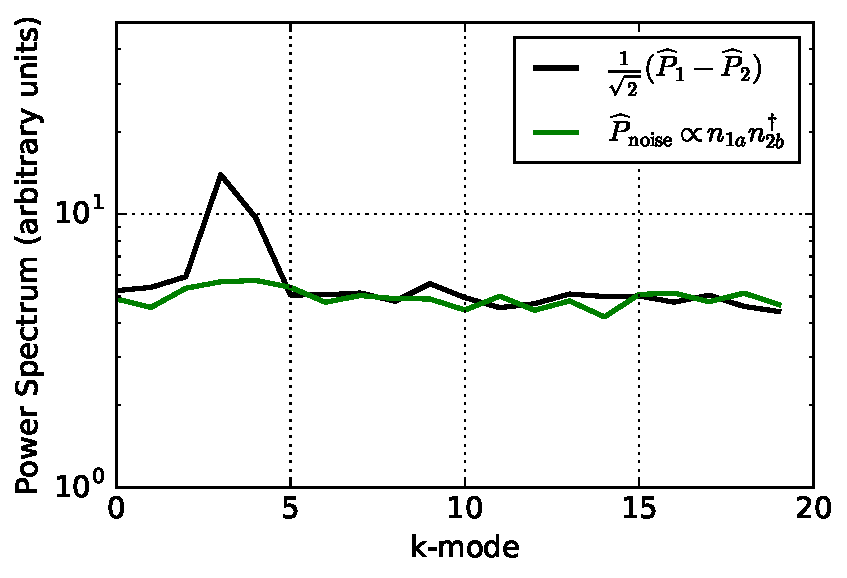
\includegraphics[trim={0cm 0cm 0cm 0cm},width=0.65\textwidth]{plots/toy_bias1.pdf}
	\caption{A null jackknife test shown as the power spectrum difference between two measurements (black), compared to the power spectrum of noise alone (green). Because the null test is not consistent with noise, it suggests the 
presence of a systematic in either $\textbf{x}_{1}$ or $\textbf{x}_{2}$. Null tests of clean measurements should be consistent 
with thermal noise.}
	\label{fig:toy_bias1}
\end{figure}

\begin{figure}
	\centering
	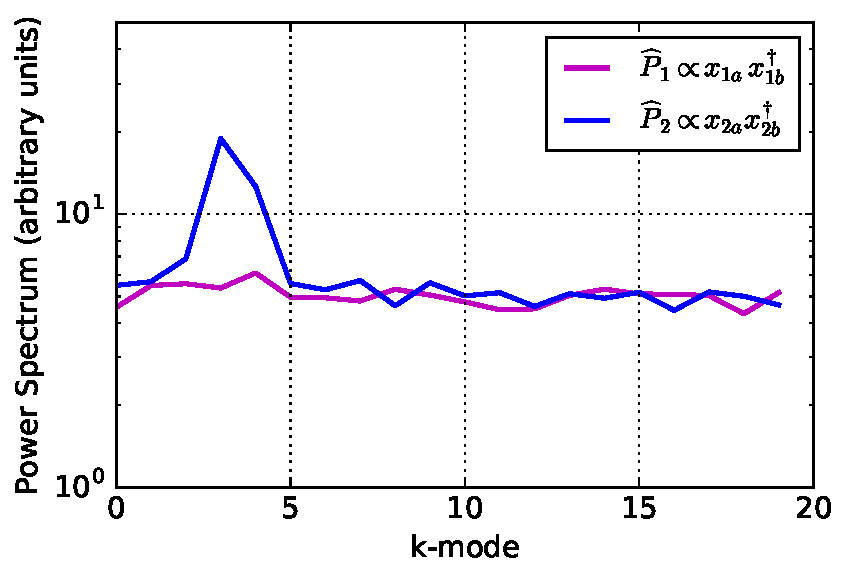
\includegraphics[trim={0cm 0cm 0cm 0cm},width=0.65\textwidth]{plots/toy_bias2.pdf}
	\caption{Power spectrum estimates for $\textbf{x}_{1}$ and $\textbf{x}_{2}$, two jackknives of the toy model. They suggest 
the presence of a systematic in $\textbf{x}_{2}$ only, illustrating how jackknives can be used to tease out excesses. Clean 
measurements should remain consistent despite the jackknife taken.}
	\label{fig:toy_bias2}
\end{figure}

We do not perform a time-average or apply a fringe-rate filter to this toy model, since we are interested only in what jackknife 
tests can tell us about biases. For the same reason, we use a weighting matrix of $\textbf{I}$ for power spectrum estimation to 
avoid signal loss. 

To construct a null test, we difference the two power spectra, with the result shown in Figure \ref{fig:toy_bias1} (black) along with the power spectrum of noise only (green). Subtracting the two estimates removes sky signal that should ideally be present in both jackknives. However, we see a clear difference between the null test and the power spectrum of 
noise. This signifies a non-EoR bias that is only present in either $\textbf{x}_{1}$ or $\textbf{x}_{2}$, but not both.

While the null test is useful for testing noise properties and the uniformity of a dataset, jackknives are useful in pinpointing 
which data subsets are contaminated by biases and which are not; in our toy model we see that the bias exists only in $
\textbf{x}_{2}$ (Figure \ref{fig:toy_bias2}). If foreground or noise biases exist in a dataset, jackknives can tease them out and 
provide insight into possible sources. For example, if jackknives along the time-axis reveal a bias present at a certain LST, a 
likely explanation would be excess foreground emission from a radio source in the sky at that time. A jackknife test involving 
data before and after the application of a fringe-rate filter can reveal whether crosstalk noise bias is successfully suppressed 
with the filter, or if similar-shaped detections in both power spectra suggest otherwise. There are many other jackknife axes of 
which we will not go into detail here, including baseline, frequency, and polarization. Ultimately, an EoR detection should persist 
through them all and a clean measurement should exhibit noise-like null spectra.

In this section we have highlighted how null tests and jackknife tests are key for determining the nature of a power spectrum 
detection. In Chapter \ref{sec:Bias} we perform some examples of these tests on PAPER-64 data in order to show that our 
excesses are not EoR and to identify their likely cause. 




